\documentclass[conference]{IEEEtran}

\usepackage[T1]{fontenc}
\usepackage[utf8]{inputenc}
\usepackage{pgfplots}
\pgfplotsset{compat=1.18}
\usepackage{tikz}
\usetikzlibrary{shapes.geometric, arrows.meta, positioning, calc, decorations.pathreplacing, patterns, fit}
\usepackage{booktabs}
\usepackage{array}
\usepackage{hyperref}
\usepackage{xcolor}
\usepackage{graphicx}
\usepackage{float}
\usepackage{enumitem}
\usepackage{amsmath}
\usepackage{amssymb}
\usepackage{balance}
\usepackage{listings}
\usepackage{multirow}
\usepackage{tabularx}
\usepackage{algorithm}
\usepackage{algorithmic}
\usepackage{cite}
\usepackage{url}
\usepackage{pifont}
\usepackage{subcaption}

\definecolor{ieeblue}{HTML}{1A5276}
\definecolor{accent}{HTML}{C0392B}
\definecolor{chartblue}{HTML}{2874A6}
\definecolor{chartgreen}{HTML}{1E8449}
\definecolor{chartorange}{HTML}{CA6F1E}
\definecolor{chartred}{HTML}{C0392B}
\definecolor{chartpurple}{HTML}{6C3483}
\definecolor{chartgray}{HTML}{5D6D7E}
\definecolor{chartteal}{HTML}{148F77}
\definecolor{inkcolor}{HTML}{0D0D0D}
\definecolor{papercolor}{HTML}{F2EFE9}
\definecolor{accentred}{HTML}{E8341A}
\definecolor{codebg}{HTML}{F5F5F5}

\hypersetup{
    colorlinks=true,
    linkcolor=ieeblue,
    urlcolor=ieeblue,
    citecolor=ieeblue
}

\lstset{
    basicstyle=\ttfamily\scriptsize,
    backgroundcolor=\color{codebg},
    frame=single,
    framerule=0.4pt,
    rulecolor=\color{gray!40},
    breaklines=true,
    columns=fullflexible,
    keepspaces=true,
    showstringspaces=false,
    tabsize=2,
    xleftmargin=4pt,
    xrightmargin=4pt,
    aboveskip=4pt,
    belowskip=4pt,
    numbers=left,
    numberstyle=\tiny\color{gray},
    numbersep=5pt,
    keywordstyle=\color{ieeblue}\bfseries,
    stringstyle=\color{chartgreen},
    commentstyle=\color{chartgray}\itshape,
    language=Java,
}

\begin{document}

\title{A Scalable Self-Service Platform for Constraint-Enforced\\Cross-Disciplinary Team Formation in\\Engineering Education}

\author{
\IEEEauthorblockN{Mithun Gowda B\textsuperscript{1}, Harsha N\textsuperscript{2}, Naren V\textsuperscript{3}, Nevil Anson Dsouza\textsuperscript{4}}
\IEEEauthorblockA{Department of Computer Science and Engineering\\
Don Bosco Institute of Technology, Bangalore, India\\
Visvesvaraya Technological University (VTU)\\
\{mithungowda.b7411, harsha210108, narenbhaskar2007, nevilansondsouza\}@gmail.com}
}

\maketitle

% ============================================================
\begin{abstract}
% ============================================================
Cross-disciplinary team formation is a critical yet underserved challenge in engineering education. Institutions must organize hundreds or thousands of students into balanced, diverse teams that satisfy pedagogical constraints---a process that is time-consuming when done manually, inflexible when done algorithmically, and unsupported by existing Learning Management Systems. This paper presents a novel self-service team formation platform that combines \textit{student agency} with \textit{automated real-time constraint enforcement}---a hybrid approach absent from current solutions. The system enables students to create teams, invite members, and browse open teams, while a constraint engine enforces configurable diversity rules (e.g., branch concentration limits, minimum diversity thresholds, mandatory representation requirements) at every stage of team composition. We formalize the constraint model with four parameterizable rules, present a two-phase race-condition-safe validation algorithm with formal complexity analysis, and describe a five-layer defense-in-depth security architecture including custom email-based OTP authentication, JWT sessions, document-level access control, and IP-based rate limiting. A six-layer duplication prevention framework guarantees data integrity invariants---preventing duplicate team memberships, redundant invitations, and orphaned references. A multi-key email delivery system with round-robin load balancing and automatic failover enables operation within free-tier email quotas. The platform is implemented as an open-source Next.js application with Firebase Firestore, comprising 8,245 lines of TypeScript across 58 files. We validate the approach through a production deployment at an Indian engineering institution serving 823 students across 7 branches, and present a comparative analysis against five existing team formation approaches across 13 evaluation criteria. Results demonstrate an estimated 96\% reduction in administrative effort, 100\% constraint satisfaction for completed teams, sub-second real-time constraint feedback, and zero data integrity violations. The architecture is generalizable to any institution with configurable branch structures, team sizes, and diversity policies, deployable at zero operational cost on serverless infrastructure.
\end{abstract}

\begin{IEEEkeywords}
Team Formation, Cross-Disciplinary Education, Constraint Validation, Self-Service Platform, Engineering Education, Real-Time Web Application, Data Integrity, Duplication Prevention, Open Source
\end{IEEEkeywords}

% ============================================================
\section{Introduction}
\label{sec:introduction}
% ============================================================

\subsection{The Team Formation Challenge in Engineering Education}

Interdisciplinary collaboration is a cornerstone of modern engineering education. The Accreditation Board for Engineering and Technology (ABET) explicitly requires that graduates ``function effectively on teams that establish goals, plan tasks, meet deadlines, and analyze risk and uncertainty''~\cite{abet2019}. Research consistently demonstrates that collaborative, cross-disciplinary learning produces measurable gains in problem-solving, communication, and systems thinking~\cite{terenzini2001, borrego2010}. Prince~\cite{prince2004} provides a comprehensive review showing that active learning pedagogies---including team-based project work---produce statistically significant improvements in student performance compared to traditional lecture-based instruction. As a result, project-based learning with diverse teams has become standard practice across engineering curricula worldwide.

However, \textit{forming} these teams at scale remains a significant operational challenge that has received insufficient attention in the literature. Consider a typical large engineering institution with 500--2,000 first-year students across 5--10 branches. Forming teams of 4--8 members that satisfy branch diversity constraints requires:

\begin{itemize}[noitemsep,topsep=3pt]
    \item Organizing hundreds of students into $\sim$100--300 teams
    \item Enforcing diversity constraints (e.g., no more than $k$ members from any single branch, minimum $d$ unique branches per team, mandatory representation from specific branches)
    \item Managing iterative team building over days or weeks as students join at different times
    \item Handling invitations, join requests, approvals, and rejections across hundreds of concurrent interactions
    \item Preventing data integrity violations: duplicate team memberships, conflicting invitations, orphaned registrations, and race conditions during concurrent operations
    \item Providing administrative oversight with real-time monitoring and intervention capabilities
\end{itemize}

Existing approaches to this problem fall into three categories, each with significant limitations (Table~\ref{tab:approaches}):

\begin{table}[htbp]
\centering
\caption{Limitations of Existing Team Formation Approaches}
\label{tab:approaches}
\footnotesize
\renewcommand{\arraystretch}{1.15}
\begin{tabular}{@{}p{1.5cm}p{2.5cm}p{2.5cm}@{}}
\toprule
\textbf{Approach} & \textbf{Method} & \textbf{Key Limitations} \\
\midrule
Manual & Spreadsheets, email coordination & Days of effort, constraint violations, no real-time validation, duplicate assignments \\
Algorithmic & Batch optimization (e.g., CATME~\cite{ohland2012}) & No student agency, batch-only, no iterative building \\
LMS-based & Moodle groups, Canvas teams~\cite{moodle} & No constraint enforcement, no diversity validation, partial duplicate prevention \\
\bottomrule
\end{tabular}
\end{table}

\subsection{The Data Integrity Problem}

Beyond the team formation challenge itself, a critical but often overlooked problem is \textbf{data integrity during self-service team formation}. When hundreds of students concurrently create teams, send invitations, and process join requests, numerous integrity violations can occur: a student may be assigned to multiple teams simultaneously, the same invitation may be issued twice, concurrent acceptance operations may corrupt team rosters, and team dissolution may leave orphaned membership records that block future team joining. Manual processes are particularly susceptible to these issues---spreadsheet-based coordination routinely produces duplicate assignments that require hours of post-hoc correction~\cite{felder2000}. Even LMS platforms like Moodle only partially address duplication: they prevent duplicate \textit{group enrollment} but do not guard against duplicate invitations, redundant join requests, or cascade-cleanup failures.

\subsection{Research Gap}

The fundamental gap across existing solutions is the absence of a system that combines \textbf{student self-selection} (preserving agency and motivation~\cite{chapman2006}) with \textbf{real-time automated constraint enforcement} (guaranteeing diversity requirements~\cite{oakley2004}) and \textbf{comprehensive data integrity guarantees} (eliminating duplication and orphaned state). This gap is illustrated in Fig.~\ref{fig:gap}.

\begin{figure}[htbp]
\centering
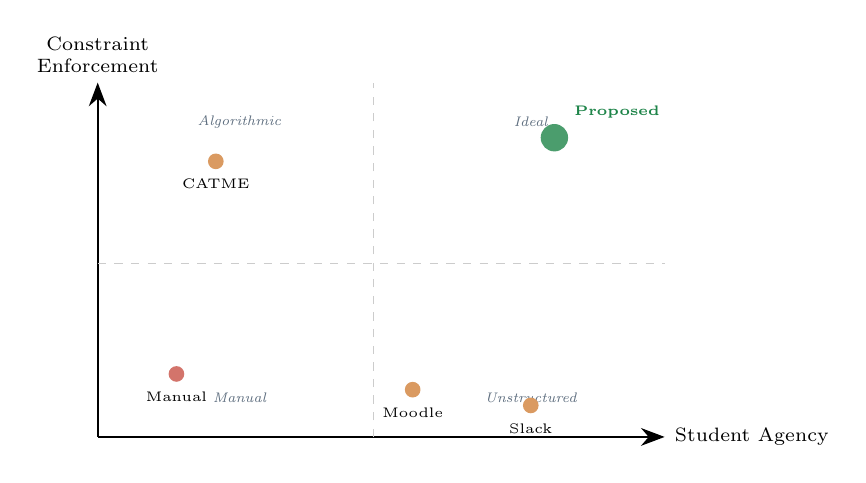
\begin{tikzpicture}[
    every node/.style={font=\small},
    box/.style={draw, rounded corners=4pt, minimum width=2cm, minimum height=1cm, align=center, line width=0.6pt}
]
    % Axes
    \draw[-{Stealth[length=3mm]}, thick] (0,0) -- (7.2,0) node[right, font=\scriptsize] {Student Agency};
    \draw[-{Stealth[length=3mm]}, thick] (0,0) -- (0,4.5) node[above, font=\scriptsize, align=center] {Constraint\\Enforcement};

    % Quadrant labels
    \node[font=\tiny\itshape, color=chartgray] at (1.8, 4.0) {Algorithmic};
    \node[font=\tiny\itshape, color=chartgray] at (5.5, 4.0) {Ideal};
    \node[font=\tiny\itshape, color=chartgray] at (1.8, 0.5) {Manual};
    \node[font=\tiny\itshape, color=chartgray] at (5.5, 0.5) {Unstructured};

    % Existing solutions
    \node[circle, fill=chartred!70, inner sep=2pt, label={[font=\tiny]below:Manual}] at (1.0, 0.8) {};
    \node[circle, fill=chartorange!70, inner sep=2pt, label={[font=\tiny]below:CATME}] at (1.5, 3.5) {};
    \node[circle, fill=chartorange!70, inner sep=2pt, label={[font=\tiny]below:Moodle}] at (4.0, 0.6) {};
    \node[circle, fill=chartorange!70, inner sep=2pt, label={[font=\tiny]below:Slack}] at (5.5, 0.4) {};

    % Our solution
    \node[circle, fill=chartgreen!80, inner sep=3.5pt, label={[font=\tiny\bfseries, color=chartgreen]above right:Proposed}] at (5.8, 3.8) {};

    % Dashed lines for quadrants
    \draw[dashed, gray!40] (3.5, 0) -- (3.5, 4.5);
    \draw[dashed, gray!40] (0, 2.2) -- (7.2, 2.2);
\end{tikzpicture}
\caption{Positioning of team formation approaches along student agency and constraint enforcement dimensions. Existing solutions cluster in three quadrants; the upper-right quadrant (high agency + high enforcement) remains unoccupied.}
\label{fig:gap}
\end{figure}

\subsection{Contributions}

This paper makes the following contributions:

\begin{enumerate}[noitemsep,topsep=3pt]
    \item A \textbf{hybrid team formation model} (Section~\ref{sec:model}) that preserves student self-selection while enforcing institutional constraints in real time---occupying the previously unserved upper-right quadrant of Fig.~\ref{fig:gap}

    \item A \textbf{formal constraint specification and validation algorithm} (Section~\ref{sec:constraints}) with configurable diversity rules, complexity analysis, and race-condition protection through server-side re-validation

    \item A \textbf{six-layer duplication prevention framework} (Section~\ref{subsec:duplication}) ensuring single-team membership, invite idempotency, and cascade cleanup---guaranteeing data integrity across all concurrent operations

    \item A \textbf{five-layer security architecture} (Section~\ref{sec:security}) combining email-based OTP authentication, JWT sessions, Firebase custom tokens, document-level access control, and IP-based rate limiting---designed for environments where students lack institutional SSO credentials

    \item A \textbf{comprehensive comparative evaluation} (Section~\ref{sec:comparison}) against five existing approaches across 13 criteria, demonstrating advantages in constraint satisfaction, data integrity, real-time feedback, and administrative efficiency

    \item A \textbf{production validation} (Section~\ref{sec:casestudy}) at an engineering institution with 823 students across 7 branches, demonstrating practical viability at institutional scale with quantitative performance measurements

    \item A complete \textbf{open-source implementation} (8,245 lines of TypeScript, 58 files) deployable on serverless infrastructure with zero operational cost on free tiers
\end{enumerate}

% ============================================================
\section{Related Work}
\label{sec:related}
% ============================================================

\subsection{Instructor-Driven Team Formation}

Oakley et al.~\cite{oakley2004} provide comprehensive guidelines for instructor-formed teams, recommending heterogeneous groupings based on academic performance and schedule compatibility. Their study of engineering courses found that instructor-formed heterogeneous teams consistently outperformed student-selected homogeneous teams on project outcomes. The CATME system~\cite{ohland2012} automates this approach using student surveys covering schedules, GPA, demographics, and personality characteristics. CATME's Team-Maker module uses a constraint satisfaction algorithm that optimizes team composition across multiple criteria simultaneously, and has been adopted by over 2,000 institutions worldwide.

However, instructor-driven approaches share two fundamental limitations. First, they require significant instructor effort for each cohort---even with automation, instructors must design survey instruments, configure optimization parameters, resolve edge cases, and handle student complaints about assignments. Second, and more critically, they \textit{entirely eliminate student agency in teammate selection}. Chapman et al.~\cite{chapman2006} demonstrate that this loss of agency is strongly correlated with reduced team satisfaction and lower intrinsic motivation, as students perceive imposed teams as arbitrary constraints rather than collaborative partnerships.

Felder and Brent~\cite{felder2000} recommend a middle ground---providing guidelines for team formation while allowing some student input---but do not provide a systematic mechanism for enforcing this balance at scale. Their work acknowledges the tension between instructor control and student agency but offers no technical solution.

\subsection{Student Self-Selection}

Chapman et al.~\cite{chapman2006} provide the strongest empirical evidence for self-selection: in a controlled study across 16 undergraduate course sections, student-selected teams reported significantly higher satisfaction ($p < 0.01$), stronger interpersonal cohesion ($p < 0.05$), and greater willingness to work together in the future ($p < 0.01$) compared to instructor-assigned teams. However, Bacon et al.~\cite{bacon2004} identify a critical limitation: self-selected teams exhibit \textbf{homogeneity bias}, gravitating toward same-branch, same-background groupings that undermine the pedagogical goals of cross-disciplinary exposure. Their longitudinal study of 508 team experiences found that the ``worst'' team experiences were disproportionately associated with self-selected homogeneous groups that lacked complementary skills.

Smith and MacGregor~\cite{smith1992} provide a theoretical framework for collaborative learning that emphasizes the importance of \textit{cognitive diversity}---the variety of perspectives and problem-solving approaches within a team. When self-selection produces homogeneous teams, this cognitive diversity is lost, reducing the learning benefits that motivated team-based pedagogy in the first place. Without structural enforcement, self-selection produces teams that are socially comfortable but academically suboptimal.

\subsection{Algorithmic Approaches}

Lappas et al.~\cite{lappas2009} formalize team formation as a constrained optimization problem and establish its NP-hardness for the general case where both team quality and inter-member communication cost must be optimized simultaneously. Their social-network-based approach minimizes communication cost subject to skill coverage constraints, using approximation algorithms with provable guarantees.

Anagnostopoulos et al.~\cite{anagnostopoulos2012} extend this to \textit{online} settings where team members arrive sequentially and assignments are irrevocable---a model closer to educational team formation where students register over a period of days. Their analysis shows that online algorithms achieve competitive ratios within constant factors of offline optima for many practical constraint structures.

Wi et al.~\cite{wi2009} apply genetic algorithms to optimize team competency coverage in R\&D settings, demonstrating that evolutionary approaches can handle complex multi-objective constraints. While algorithmically sophisticated, all these approaches treat students as passive inputs to an optimization function, completely removing agency from the process. Furthermore, none provide real-time feedback during team building---they operate in batch mode, computing assignments after all preferences have been collected.

\subsection{Learning Management Systems}

Moodle~\cite{moodle} supports three group modes: (1)~random assignment, which distributes students across groups without constraint consideration; (2)~manual assignment by instructors, which provides control but no automation; and (3)~self-selection, which allows students to join groups but provides no constraint enforcement, validation, or real-time feedback. Canvas offers similar group functionality with marginally better UI but identical lack of constraint support. Google Classroom and Microsoft Teams support group creation but lack validation for diversity requirements entirely.

Critically, while Moodle prevents students from being in multiple instances of the same group set, it does \textit{not} prevent duplicate invitations, redundant join requests, or the cascade-cleanup issues that arise when groups are dissolved. The partial duplication prevention offered by LMS platforms is insufficient for the complex invitation/request workflows that characterize self-service team formation.

\subsection{Real-Time Web Platforms}

Modern real-time platforms (Slack, Discord, GitHub Teams) enable informal collaboration but lack the structured constraint enforcement required for educational team formation. Students can create channels and invite peers, but there is no mechanism to enforce branch composition rules, prevent over-concentration from a single discipline, or guarantee that mandatory representation requirements are met. These platforms also provide no administrative oversight tools---instructors cannot monitor team composition, enforce deadlines, or intervene in the formation process.

Firebase Firestore~\cite{firebase} provides real-time database subscriptions that enable reactive user interfaces---a capability we leverage for instant constraint feedback and notifications. Unlike traditional REST APIs that require polling, Firestore's \texttt{onSnapshot()} listeners push data changes to all connected clients within milliseconds, enabling the real-time constraint validation that is central to our approach.

\subsection{Summary of Gap}

Table~\ref{tab:gapsummary} synthesizes the capabilities of existing approaches. No existing system combines student self-selection with automated, real-time constraint enforcement and comprehensive data integrity guarantees. Our platform fills this gap by providing a structured self-service environment where students freely choose teammates while the system guarantees every completed team satisfies institutional diversity requirements and no data integrity violations occur.

\begin{table}[htbp]
\centering
\caption{Capability Gap Analysis of Existing Approaches}
\label{tab:gapsummary}
\footnotesize
\renewcommand{\arraystretch}{1.15}
\begin{tabular}{@{}lcccc@{}}
\toprule
\textbf{Capability} & \textbf{Manual} & \textbf{Algo.} & \textbf{LMS} & \textbf{Ours} \\
\midrule
Student agency & \ding{55} & \ding{55} & \checkmark & \checkmark \\
Constraint enforcement & \ding{55} & \checkmark & \ding{55} & \checkmark \\
Real-time feedback & \ding{55} & \ding{55} & \ding{55} & \checkmark \\
Iterative building & \checkmark & \ding{55} & \checkmark & \checkmark \\
Duplicate prevention & \ding{55} & \checkmark & Partial & \checkmark \\
Admin oversight & \ding{55} & \checkmark & \checkmark & \checkmark \\
Zero cost & \checkmark & \ding{55} & \ding{55} & \checkmark \\
\bottomrule
\end{tabular}
\end{table}

% ============================================================
\section{Hybrid Team Formation Model}
\label{sec:model}
% ============================================================

\subsection{Design Principles}

The platform is designed around five principles derived from the literature:

\begin{enumerate}[noitemsep,topsep=3pt]
    \item \textbf{Student agency:} Students initiate team creation, select teammates, and choose which teams to join---preserving the motivational benefits of self-selection~\cite{chapman2006}
    \item \textbf{Automated constraint enforcement:} Every member addition is validated against institutional diversity rules in real time, eliminating the homogeneity bias of pure self-selection~\cite{bacon2004}
    \item \textbf{Progressive guidance:} Soft warnings guide students toward constraint satisfaction during intermediate team building stages, with hard blocks only at the point of violation or team completion
    \item \textbf{Data integrity by design:} Duplication prevention, idempotent operations, and cascade cleanup are built into every state transition, not bolted on after the fact
    \item \textbf{Administrative oversight:} Gate controls, bulk data management, real-time statistics, and intervention capabilities provide institutional control without micromanagement
\end{enumerate}

\subsection{Workflow Model}

The team formation process follows four phases (Fig.~\ref{fig:workflow}):

\begin{figure}[htbp]
\centering
\resizebox{0.95\columnwidth}{!}{%
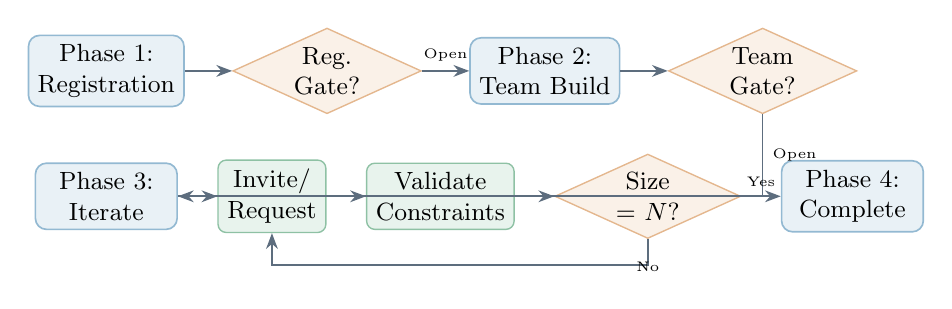
\begin{tikzpicture}[
    node distance=0.4cm and 0.5cm,
    every node/.style={font=\small},
    phase/.style={draw, rounded corners=4pt, minimum width=1.8cm, minimum height=0.7cm, align=center, fill=chartblue!10, draw=chartblue!50, line width=0.6pt},
    gate/.style={draw, diamond, aspect=2.2, minimum width=1cm, align=center, fill=chartorange!10, draw=chartorange!50, line width=0.5pt, inner sep=1pt, font=\small},
    act/.style={draw, rounded corners=3pt, minimum width=1.3cm, minimum height=0.5cm, align=center, fill=chartgreen!10, draw=chartgreen!50, line width=0.5pt},
    arrow/.style={-{Stealth[length=2mm]}, draw=chartgray, semithick}
]
    % Phase 1
    \node[phase] (reg) {Phase 1:\\Registration};
    \node[gate, right=0.6cm of reg] (reggate) {Reg.\\Gate?};

    % Phase 2
    \node[phase, right=0.6cm of reggate] (team) {Phase 2:\\Team Build};
    \node[gate, right=0.6cm of team] (teamgate) {Team\\Gate?};

    % Phase 3
    \node[phase, below=0.7cm of reg] (grow) {Phase 3:\\Iterate};
    \node[act, right=0.5cm of grow] (invite) {Invite/\\Request};
    \node[act, right=0.5cm of invite] (validate) {Validate\\Constraints};
    \node[gate, right=0.5cm of validate] (full) {Size\\= $N$?};

    % Phase 4
    \node[phase, right=0.5cm of full] (done) {Phase 4:\\Complete};

    % Arrows
    \draw[arrow] (reg) -- (reggate);
    \draw[arrow] (reggate) -- node[above, font=\tiny] {Open} (team);
    \draw[arrow] (team) -- (teamgate);
    \draw[arrow] (teamgate) |- node[right, near start, font=\tiny] {Open} (grow);
    \draw[arrow] (grow) -- (invite);
    \draw[arrow] (invite) -- (validate);
    \draw[arrow] (validate) -- (full);
    \draw[arrow] (full) -- node[above, font=\tiny] {Yes} (done);
    \draw[arrow] (full) |- node[below, near start, font=\tiny] {No} ([yshift=-0.4cm]invite.south) -- (invite);
\end{tikzpicture}%
}
\caption{Four-phase team formation workflow with administrative gate controls between phases. Phase~3 iterates until the team reaches the required size $N$ with all constraints satisfied.}
\label{fig:workflow}
\end{figure}

\textbf{Phase 1 (Registration):} Students authenticate via email OTP and register on the platform. The system validates their University Seat Number (USN) against the institution's enrollment database using configurable regex patterns and section-mapping rules. An admin-controlled registration gate enables phased enrollment---administrators can open registration before team formation begins, ensuring a critical mass of students is available when team building starts.

\textbf{Phase 2 (Team Initiation):} Students create new teams (generating a unique human-readable team code) or browse existing open teams. A separate team formation gate controls when this phase becomes available. The system assigns the team creator as the ``team lead'' with invite and management privileges.

\textbf{Phase 3 (Iterative Building):} This is the core formation phase with two parallel interaction modes:

\begin{itemize}[noitemsep,topsep=3pt]
    \item \textbf{Invite mode:} Team leads invite specific students by USN. The system validates that the target student exists, is registered, is not already on another team, and does not have a pending invite from this team. If valid, the invitation is created and the target receives an in-app notification and email.
    \item \textbf{Request mode:} Students browse open teams, view their current composition and constraint status, and submit join requests. The system validates that the requester is not already on a team and does not have a pending request for this team.
\end{itemize}

Every member addition---whether via invite acceptance or request approval---passes through the constraint engine (Section~\ref{sec:constraints}) and the duplication prevention framework (Section~\ref{subsec:duplication}) before being committed to the database.

\textbf{Phase 4 (Completion):} When a team reaches $N$ members with all constraints satisfied, it is marked complete. The full composition validation (Algorithm~\ref{alg:validate}) ensures every constraint is met. Completed teams remain visible but no longer accept new members.

\subsection{Dual-Interaction Team Building}

A distinctive feature of the platform is its \textbf{dual-interaction model}: team leads actively recruit (invite mode) while unaffiliated students proactively seek teams (browse/request mode). This dual approach addresses the ``cold-start problem'' where early-registering students have few teams to browse. Team leads can seed their teams through invitations while simultaneously receiving join requests from browsers.

The browse interface displays each team's current composition, branch distribution, open slots, and constraint status---enabling informed decision-making. Students can see which teams need members from their branch (addressing a mandatory representation requirement, for instance) and submit targeted requests, creating a marketplace-like dynamic where supply (students) and demand (team slots with specific branch needs) naturally equilibrate.

\subsection{Administrative Control Layer}

The admin interface provides three categories of control:

\begin{enumerate}[noitemsep,topsep=3pt]
    \item \textbf{Gate management:} Independent toggles for the registration gate and team formation gate, enabling administrators to orchestrate phased rollouts (e.g., open registration on Monday, open team formation on Wednesday)
    \item \textbf{Data management:} CSV bulk upload of student enrollment data, individual student management (add, modify, remove), and team intervention capabilities (remove members, dissolve teams, transfer team lead)
    \item \textbf{Real-time monitoring:} Statistics dashboard showing registration counts, team counts by status (forming, complete), branch distribution across teams, unaffiliated student counts, and constraint violation alerts
\end{enumerate}

% ============================================================
\section{Constraint Specification and Validation}
\label{sec:constraints}
% ============================================================

\subsection{Formal Constraint Model}

Let $T = \{m_1, m_2, \ldots, m_n\}$ be a team where each member $m_i$ has branch $b(m_i) \in \mathcal{B}$ for a set of branches $\mathcal{B}$. The constraint model is parameterized by four configurable values:

\begin{itemize}[noitemsep,topsep=3pt]
    \item $N \in \mathbb{Z}^+$: Required team size (e.g., 6)
    \item $K \in \mathbb{Z}^+$: Maximum members from any single branch (e.g., 4), where $K < N$
    \item $D \in \mathbb{Z}^+$: Minimum number of unique branches represented (e.g., 2), where $D \leq |\mathcal{B}|$
    \item $\mathcal{R} \subseteq \mathcal{B}$: Set of branches requiring mandatory representation (e.g., \{ECE, EEE\})
\end{itemize}

Define the branch distribution function:
\begin{equation}
    \delta(T, \beta) = |\{m_i \in T : b(m_i) = \beta\}|
\end{equation}

the diversity measure:
\begin{equation}
    U(T) = |\{\beta \in \mathcal{B} : \delta(T, \beta) > 0\}|
\end{equation}

and the branch concentration ratio:
\begin{equation}
    \gamma(T) = \frac{\max_{\beta \in \mathcal{B}} \delta(T, \beta)}{|T|}
\end{equation}

A team $T$ is \textit{valid} (i.e., satisfies all institutional constraints) if and only if:
\begin{align}
    \mathcal{C}_1(T) &: |T| = N \label{eq:c1} \\
    \mathcal{C}_2(T) &: \max_{\beta \in \mathcal{B}} \delta(T, \beta) \leq K \label{eq:c2} \\
    \mathcal{C}_3(T) &: U(T) \geq D \label{eq:c3} \\
    \mathcal{C}_4(T) &: \forall \beta \in \mathcal{R},\; \exists\, m_i \in T : b(m_i) = \beta \label{eq:c4}
\end{align}

\begin{equation}
    \text{valid}(T) \iff \mathcal{C}_1 \wedge \mathcal{C}_2 \wedge \mathcal{C}_3 \wedge \mathcal{C}_4
\end{equation}

Note that $\mathcal{C}_4$ is strengthened compared to the initial model: it requires representation from \textit{every} branch in $\mathcal{R}$, not merely at least one. This parameterization makes the model \textbf{institution-agnostic}: any institution can configure $N$, $K$, $D$, $\mathcal{B}$, and $\mathcal{R}$ to match their specific diversity policies without code changes.

\subsection{Constraint Feasibility Analysis}

Not all parameter combinations produce feasible team configurations. For a valid team to exist, the following conditions must hold:
\begin{align}
    K &\geq \lceil N / |\mathcal{B}| \rceil \label{eq:feas1} \\
    D &\leq \min(N, |\mathcal{B}|) \label{eq:feas2} \\
    |\mathcal{R}| &\leq N \label{eq:feas3} \\
    K \cdot (D - |\mathcal{R}|) + |\mathcal{R}| &\geq N - K \cdot |\mathcal{R}| \quad \text{(if } D > |\mathcal{R}|\text{)} \label{eq:feas4}
\end{align}

Condition~(\ref{eq:feas1}) ensures that the maximum concentration limit $K$ is large enough to accommodate $N$ students even in the worst case where students are evenly distributed. Condition~(\ref{eq:feas2}) ensures the diversity requirement does not exceed the team size or available branches. The system validates these feasibility conditions at configuration time and alerts administrators to infeasible parameter combinations.

\subsection{Two-Phase Validation Algorithm}

The constraint engine implements a two-phase validation strategy that balances flexibility with strictness:

\textbf{Phase A: Pre-Addition Validation.} Before every member addition, \texttt{canAddMember()} checks whether adding a candidate with branch $\beta_c$ would violate any constraint. Hard constraints ($\mathcal{C}_1$, $\mathcal{C}_2$) block immediately at every stage. Soft constraints ($\mathcal{C}_3$, $\mathcal{C}_4$) produce warnings during intermediate stages but become hard blocks when adding the $N$-th (final) member.

\begin{algorithm}[htbp]
\caption{Pre-Addition Constraint Validation (\texttt{canAddMember})}
\label{alg:canAdd}
\footnotesize
\begin{algorithmic}[1]
\REQUIRE Approved members $T_a$, candidate branch $\beta_c$, params $N, K, D, \mathcal{R}$
\ENSURE (valid, errors, warnings)
\STATE $E \gets \emptyset$; $W \gets \emptyset$
\IF{$|T_a| \geq N$}
    \STATE $E$.add(``Team full'')
    \RETURN (false, $E$, $W$)
\ENDIF
\IF{$\delta(T_a, \beta_c) + 1 > K$}
    \STATE $E$.add(``Max $K$ from $\beta_c$'')
\ENDIF
\IF{$|T_a| + 1 = N$}
    \STATE $T' \gets T_a \cup \{$candidate$\}$
    \IF{$U(T') < D$}
        \STATE $E$.add(``Need $D$+ branches'')
    \ENDIF
    \FOR{each $\beta \in \mathcal{R}$}
        \IF{$\delta(T', \beta) = 0$}
            \STATE $E$.add(``Need member from $\beta$'')
        \ENDIF
    \ENDFOR
\ELSIF{$|T_a| + 1 \geq N - 2$}
    \STATE $T' \gets T_a \cup \{$candidate$\}$
    \FOR{each $\beta \in \mathcal{R}$}
        \IF{$\delta(T', \beta) = 0$}
            \STATE $s \gets N - |T_a| - 1$
            \STATE $W$.add(``No $\beta$ member yet, $s$ slots left'')
        \ENDIF
    \ENDFOR
\ENDIF
\RETURN ($|E| = 0$, $E$, $W$)
\end{algorithmic}
\end{algorithm}

\textbf{Phase B: Completion Validation.} When the $N$-th member is added, \texttt{validateTeamComposition()} (Algorithm~\ref{alg:validate}) enforces all four constraints simultaneously, ensuring no team reaches ``complete'' status without satisfying every rule.

\begin{algorithm}[htbp]
\caption{Full Team Composition Validation}
\label{alg:validate}
\footnotesize
\begin{algorithmic}[1]
\REQUIRE Team members $T$, params $N, K, D, \mathcal{R}$
\ENSURE (valid, errors)
\STATE $E \gets \emptyset$
\STATE $T_a \gets \{m \in T : m.\text{status} = \text{``approved''}\}$
\IF{$|T_a| \neq N$}
    \STATE $E$.add(``Team size must be $N$'')
\ENDIF
\STATE Compute branch distribution $\delta(T_a, \beta)$ for all $\beta \in \mathcal{B}$
\IF{$\max_\beta \delta(T_a, \beta) > K$}
    \STATE $E$.add(``Max $K$ from any branch exceeded'')
\ENDIF
\IF{$U(T_a) < D$}
    \STATE $E$.add(``Need at least $D$ unique branches'')
\ENDIF
\FOR{each $\beta \in \mathcal{R}$}
    \IF{$\delta(T_a, \beta) = 0$}
        \STATE $E$.add(``Missing required branch $\beta$'')
    \ENDIF
\ENDFOR
\RETURN ($|E| = 0$, $E$)
\end{algorithmic}
\end{algorithm}

\subsection{Complexity Analysis}

Both algorithms operate in $O(|T| + |\mathcal{R}|)$ time. The branch distribution computation requires one pass over the member list ($O(|T|)$) using a hash map, and the mandatory representation check iterates over $\mathcal{R}$ ($O(|\mathcal{R}|)$). Since both $|T| = N$ and $|\mathcal{R}| \leq |\mathcal{B}|$ are small constants in practice (typically $N \leq 10$ and $|\mathcal{B}| \leq 15$), the validation executes in constant time with negligible computational overhead---enabling sub-50ms client-side execution as measured in our production deployment.

The space complexity is $O(|\mathcal{B}|)$ for the branch distribution hash map, again negligible for practical instances.

\subsection{Progressive Warning System}

A key design choice is the distinction between \textbf{hard errors} and \textbf{soft warnings}:

\begin{itemize}[noitemsep,topsep=3pt]
    \item \textbf{Hard errors} (team full, branch concentration exceeded) block the addition immediately. These constraints are violated at the point of addition and cannot self-correct.
    \item \textbf{Soft warnings} (insufficient diversity, missing mandatory branch) are surfaced as advisory messages during intermediate stages. They become hard errors only when adding the \textit{final} member, because the team can still satisfy these constraints through subsequent additions.
\end{itemize}

The warning threshold is configurable: in our implementation, warnings activate when $|T_a| + 1 \geq N - 2$ (within 2 slots of completion), providing early notice without being disruptive during early team building.

\subsection{Race Condition Protection}

In a concurrent multi-user environment, two students may simultaneously attempt to join a nearly-full team. Without protection, the following violations can occur:
\begin{itemize}[noitemsep,topsep=3pt]
    \item \textbf{Size overflow:} Both additions succeed, producing a team with $N+1$ members
    \item \textbf{Constraint violation:} Both additions individually pass validation, but their combined effect violates a constraint (e.g., $K+1$ members from the same branch)
\end{itemize}

We employ a \textbf{read-before-write} pattern: immediately before writing any member addition to the database, the system re-reads the current team document and re-executes \texttt{canAddMember()} against the \textit{latest} state. This adds one extra database read per operation but guarantees constraint correctness under concurrent modification without requiring distributed locks or transaction retries.

This approach is correct because Firestore document reads within the same request observe the most recent committed write, providing read-your-writes consistency. While not equivalent to serializable transactions, this pattern is sufficient for our use case where constraint violations are the primary concern---in the rare case of a genuine race (two writes in the same millisecond), at most one will succeed and the other will be rejected on re-validation.

% ============================================================
\section{System Architecture}
\label{sec:architecture}
% ============================================================

\subsection{Three-Tier Serverless Architecture}

The platform implements a three-tier serverless architecture (Fig.~\ref{fig:architecture}) designed for zero-infrastructure deployment.

\begin{figure}[htbp]
\centering
\resizebox{\columnwidth}{!}{%
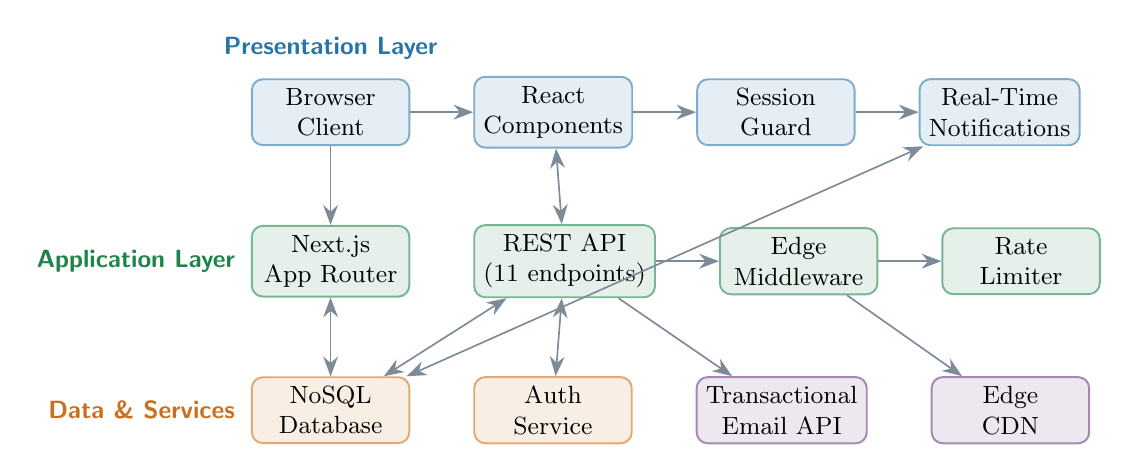
\begin{tikzpicture}[
    node distance=0.7cm and 0.8cm,
    every node/.style={font=\small},
    block/.style={draw, rounded corners=4pt, minimum width=2cm, minimum height=0.8cm, align=center, line width=0.7pt},
    client/.style={block, fill=chartblue!12, draw=chartblue!60},
    server/.style={block, fill=chartgreen!12, draw=chartgreen!60},
    db/.style={block, fill=chartorange!12, draw=chartorange!60},
    ext/.style={block, fill=chartpurple!12, draw=chartpurple!60},
    arrow/.style={-{Stealth[length=2.5mm]}, semithick, draw=chartgray!80},
    darrow/.style={{Stealth[length=2.5mm]}-{Stealth[length=2.5mm]}, semithick, draw=chartgray!80},
    lbl/.style={font=\small\bfseries\sffamily}
]
    \node[client] (browser) {Browser\\Client};
    \node[client, right=of browser] (react) {React\\Components};
    \node[client, right=of react] (session) {Session\\Guard};
    \node[client, right=of session] (notif) {Real-Time\\Notifications};

    \node[server, below=1cm of browser] (nextjs) {Next.js\\App Router};
    \node[server, right=of nextjs] (api) {REST API\\(11 endpoints)};
    \node[server, right=of api] (mw) {Edge\\Middleware};
    \node[server, right=of mw] (rate) {Rate\\Limiter};

    \node[db, below=1cm of nextjs] (firestore) {NoSQL\\Database};
    \node[db, right=of firestore] (auth) {Auth\\Service};
    \node[ext, right=of auth] (email) {Transactional\\Email API};
    \node[ext, right=of email] (cdn) {Edge\\CDN};

    \draw[arrow] (browser) -- (react);
    \draw[arrow] (react) -- (session);
    \draw[arrow] (session) -- (notif);
    \draw[arrow] (browser) -- (nextjs);
    \draw[darrow] (react) -- (api);
    \draw[arrow] (api) -- (mw);
    \draw[arrow] (mw) -- (rate);
    \draw[darrow] (nextjs) -- (firestore);
    \draw[darrow] (api) -- (firestore);
    \draw[darrow] (api) -- (auth);
    \draw[arrow] (api) -- (email);
    \draw[arrow] (mw) -- (cdn);
    \draw[darrow] (notif) -- (firestore);

    \node[lbl, color=chartblue, above=0.12cm of browser] {Presentation Layer};
    \node[lbl, color=chartgreen, left=0.08cm of nextjs, anchor=east] {Application Layer};
    \node[lbl, color=chartorange, left=0.08cm of firestore, anchor=east] {Data \& Services};
\end{tikzpicture}%
}
\caption{Three-tier serverless architecture with real-time database subscriptions enabling instant constraint feedback and notifications.}
\label{fig:architecture}
\end{figure}

The architecture is technology-agnostic in principle; our reference implementation uses Next.js~16~\cite{nextjs}, Firebase Firestore~\cite{firebase}, and Brevo Email API, but any equivalent stack (e.g., Remix + Supabase + SendGrid) could implement the same model.

\textbf{Presentation Layer.} The client is a React single-page application rendered via server-side rendering (SSR) for initial page loads and client-side navigation thereafter. The SessionGuard component implements a three-phase authentication check: (1)~local storage for cached session state, (2)~JWT and Firebase token initialization, and (3)~Firestore document verification against the registration database. Real-time notifications use Firestore's \texttt{onSnapshot()} listener with an \texttt{isInitialLoad} flag to suppress notification alerts during initial data hydration.

\textbf{Application Layer.} The Next.js App Router handles 11 REST API endpoints (Table~\ref{tab:endpoints}), each implementing input validation, authentication verification, business logic, and response formatting. Edge middleware intercepts all API requests for origin verification, security header injection, and route protection. The rate limiter operates at the IP level with configurable sliding windows.

\begin{table}[htbp]
\centering
\caption{REST API Endpoints}
\label{tab:endpoints}
\footnotesize
\renewcommand{\arraystretch}{1.1}
\begin{tabular}{@{}lll@{}}
\toprule
\textbf{Endpoint} & \textbf{Method} & \textbf{Purpose} \\
\midrule
\texttt{/auth/send-otp} & POST & Send OTP via email \\
\texttt{/auth/verify-otp} & POST & Verify OTP, issue JWT \\
\texttt{/auth/logout} & POST & Clear session \\
\texttt{/auth/session} & GET & Validate current session \\
\texttt{/auth/refresh} & POST & Refresh JWT token \\
\texttt{/admin/students} & POST & Bulk CSV upload \\
\texttt{/admin/config} & GET/POST & System configuration \\
\texttt{/admin/stats} & GET & Dashboard statistics \\
\texttt{/admin/remove-member} & POST & Remove/transfer/dissolve \\
\texttt{/admin/login} & POST & Admin authentication \\
\texttt{/notify} & POST & Email notifications \\
\bottomrule
\end{tabular}
\end{table}

\textbf{Data Layer.} Firebase Firestore provides the NoSQL document database with real-time subscriptions. Firebase Authentication provides the custom token infrastructure for client-side database access. External services include the Brevo transactional email API (with multi-key round-robin) and Vercel's Edge CDN for static asset delivery.

\subsection{Data Model}

The database uses 8 collections (Table~\ref{tab:collections}). A key design decision is \textbf{embedding member arrays within team documents} rather than using normalized junction tables. This denormalized design enables:

\begin{itemize}[noitemsep,topsep=3pt]
    \item \textbf{Single-document reads:} Complete team state (all members, branches, statuses) is retrieved in one database read, critical for real-time constraint validation
    \item \textbf{Atomic member operations:} Adding or removing a member is an atomic update to a single document, preventing partial-state issues
    \item \textbf{Efficient subscriptions:} Real-time listeners need only subscribe to one document per team, reducing subscription overhead
    \item \textbf{Natural deduplication:} Member arrays are mapped by USN, preventing duplicate entries at the data model level
\end{itemize}

\begin{table}[htbp]
\centering
\caption{Database Collections and Their Roles}
\label{tab:collections}
\footnotesize
\renewcommand{\arraystretch}{1.15}
\begin{tabular}{@{}lp{1.5cm}p{3cm}@{}}
\toprule
\textbf{Collection} & \textbf{Key} & \textbf{Purpose} \\
\midrule
\texttt{students} & Student ID & Master enrollment data from institutional CSV \\
\texttt{registrations} & Student ID & Active platform users with teamId foreign key \\
\texttt{teams} & Team code & Teams with embedded member arrays \\
\texttt{invites} & Invite code & Invites and join requests with status FSM \\
\texttt{notifications} & Auto-gen & Real-time notification documents \\
\texttt{config} & Singleton & System configuration (gates, constraints) \\
\texttt{otp\_codes} & Auto-gen & Time-limited verification codes \\
\texttt{admins} & Email hash & Admin whitelist for dashboard access \\
\bottomrule
\end{tabular}
\end{table}

\subsection{Real-Time Notification System}

The platform implements a 10-type notification system that provides real-time feedback for all team formation events:

\begin{table}[htbp]
\centering
\caption{Notification Types and Triggers}
\label{tab:notiftypes}
\footnotesize
\renewcommand{\arraystretch}{1.1}
\begin{tabular}{@{}ll@{}}
\toprule
\textbf{Notification Type} & \textbf{Trigger Event} \\
\midrule
\texttt{invite\_received} & Team lead sends invitation \\
\texttt{request\_received} & Student submits join request \\
\texttt{invite\_accepted} & Invitee accepts invitation \\
\texttt{invite\_rejected} & Invitee declines invitation \\
\texttt{request\_approved} & Team lead approves request \\
\texttt{request\_rejected} & Team lead declines request \\
\texttt{kicked\_from\_team} & Admin removes a member \\
\texttt{member\_left\_team} & Member voluntarily leaves \\
\texttt{team\_dissolved} & Admin dissolves entire team \\
\texttt{lead\_transferred} & Team lead role transferred \\
\bottomrule
\end{tabular}
\end{table}

Notifications are delivered through two channels simultaneously: (1)~in-app real-time delivery via Firestore \texttt{onSnapshot()} listeners, providing instant feedback without page refresh, and (2)~email notifications via the Brevo API for offline awareness. The \texttt{useNotifications} hook uses an \texttt{isInitialLoad} ref flag to distinguish between the initial data hydration (which should not trigger browser notification popups) and genuine new notifications (which should).

\subsection{Unambiguous ID Generation}

Team codes and invite codes are generated using a character set specifically designed to prevent visual ambiguity:

\begin{center}
\texttt{ABCDEFGHJKLMNPQRSTUVWXYZ23456789}
\end{center}

This 30-character alphabet deliberately excludes five commonly confused characters: \texttt{I} (confused with \texttt{1} and \texttt{l}), \texttt{O} (confused with \texttt{0}), \texttt{0} (confused with \texttt{O}), \texttt{1} (confused with \texttt{I} and \texttt{l}), and \texttt{L} (confused with \texttt{1} in some fonts). Team codes follow the format \texttt{TEAM-XXXX} ($30^4 = 810{,}000$ combinations) and invite codes follow \texttt{INV-XXXXXX} ($30^6 \approx 729$ million combinations), providing sufficient uniqueness for institutional-scale deployments while remaining easy to communicate verbally.

% ============================================================
\section{Data Integrity and Duplication Prevention}
\label{subsec:duplication}
% ============================================================

A critical yet often overlooked challenge in self-service team formation is \textbf{preventing data duplication}---ensuring that students cannot join multiple teams, receive duplicate invitations, or submit redundant join requests. Unlike instructor-managed approaches where a human arbiter manually resolves conflicts, a self-service platform must enforce uniqueness invariants automatically and at every entry point. Our system implements a \textbf{six-layer duplication prevention framework} (Fig.~\ref{fig:dupflow}).

\begin{figure}[htbp]
\centering
\resizebox{0.95\columnwidth}{!}{%
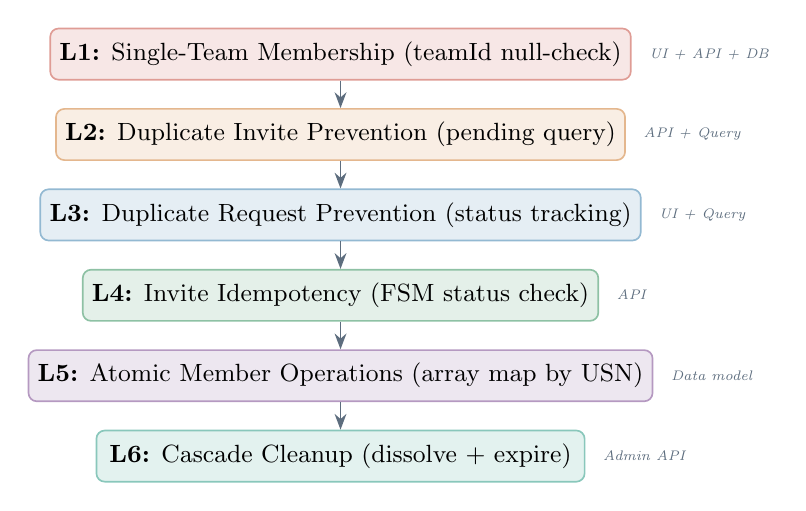
\begin{tikzpicture}[
    node distance=0.35cm,
    every node/.style={font=\small},
    layer/.style={draw, rounded corners=3pt, minimum width=6.2cm, minimum height=0.65cm, align=center, line width=0.6pt}
]
    \node[layer, fill=chartred!12, draw=chartred!50] (l1) {\textbf{L1:} Single-Team Membership (teamId null-check)};
    \node[layer, fill=chartorange!12, draw=chartorange!50, below=of l1] (l2) {\textbf{L2:} Duplicate Invite Prevention (pending query)};
    \node[layer, fill=chartblue!12, draw=chartblue!50, below=of l2] (l3) {\textbf{L3:} Duplicate Request Prevention (status tracking)};
    \node[layer, fill=chartgreen!12, draw=chartgreen!50, below=of l3] (l4) {\textbf{L4:} Invite Idempotency (FSM status check)};
    \node[layer, fill=chartpurple!12, draw=chartpurple!50, below=of l4] (l5) {\textbf{L5:} Atomic Member Operations (array map by USN)};
    \node[layer, fill=chartteal!12, draw=chartteal!50, below=of l5] (l6) {\textbf{L6:} Cascade Cleanup (dissolve + expire)};

    \draw[-{Stealth[length=2mm]}, semithick, chartgray] (l1) -- (l2);
    \draw[-{Stealth[length=2mm]}, semithick, chartgray] (l2) -- (l3);
    \draw[-{Stealth[length=2mm]}, semithick, chartgray] (l3) -- (l4);
    \draw[-{Stealth[length=2mm]}, semithick, chartgray] (l4) -- (l5);
    \draw[-{Stealth[length=2mm]}, semithick, chartgray] (l5) -- (l6);

    \node[font=\tiny\itshape, color=chartgray, right=0.1cm of l1] {UI + API + DB};
    \node[font=\tiny\itshape, color=chartgray, right=0.1cm of l2] {API + Query};
    \node[font=\tiny\itshape, color=chartgray, right=0.1cm of l3] {UI + Query};
    \node[font=\tiny\itshape, color=chartgray, right=0.1cm of l4] {API};
    \node[font=\tiny\itshape, color=chartgray, right=0.1cm of l5] {Data model};
    \node[font=\tiny\itshape, color=chartgray, right=0.1cm of l6] {Admin API};
\end{tikzpicture}%
}
\caption{Six-layer duplication prevention framework. Each layer prevents a specific class of data integrity violation.}
\label{fig:dupflow}
\end{figure}

\subsection{L1: Single-Team Membership Enforcement}

Each student's registration document contains a \texttt{teamId} field that serves as a single-assignment constraint. Before \textit{any} team join operation---whether via invitation acceptance, join-request approval, or team creation---the system verifies that \texttt{teamId} is \texttt{null}. This check is enforced at \textbf{three independent levels}:

\begin{enumerate}[noitemsep,topsep=3pt]
    \item \textbf{Client-side UI guards:} React components conditionally render ``You're already on a team'' messages and disable join/create buttons when \texttt{session.teamId} is non-null. This provides immediate user feedback without server round-trips.
    \item \textbf{Application-logic validation:} The InviteManager component queries the target student's registration document and rejects invitations with ``This student is already on another team'' if \texttt{regData.teamId} is set. The browse page rejects join requests with ``You're already on a team'' if the session has a team assignment.
    \item \textbf{Database security rules:} Firestore rules restrict \texttt{teamId} and \texttt{teamRole} updates to: (a)~the student themselves updating their own document, or (b)~a verified team lead setting these fields for a member of their team. Direct database writes that bypass the API are blocked.
\end{enumerate}

This \textbf{defense-in-depth} approach ensures that even if client-side validation is bypassed (e.g., via browser developer tools), the server-side and database-level checks reject unauthorized membership changes.

\subsection{L2: Duplicate Invite Prevention}

Before the team lead can issue an invitation, the system executes three sequential checks:

\begin{enumerate}[noitemsep,topsep=3pt]
    \item \textbf{Existing member check:} The system verifies that the target USN is not already in the team's member array, preventing redundant invites to current team members.
    \item \textbf{Pending invite check:} The system queries the \texttt{invites} collection for any document matching \texttt{(toUSN, teamId, type=``invite'', status=``pending'')}. If a pending invite already exists, the operation is rejected with ``An invite is already pending for this student.''
    \item \textbf{Cross-team membership check:} The system reads the target student's registration document and verifies that \texttt{teamId} is \texttt{null}, preventing invites to students who are already on another team.
\end{enumerate}

These checks prevent three classes of wasteful invitations: inviting existing members, duplicating pending invites, and inviting unavailable students.

\subsection{L3: Duplicate Join-Request Prevention}

Symmetrically, when a student requests to join a team via the browse interface, the system executes a compound Firestore query for any existing document matching \texttt{(fromUSN, teamId, type=``request'', status=``pending'')}. If found, the request button renders ``Request Pending'' instead of allowing a duplicate submission. The system also tracks \texttt{rejected} requests separately, displaying ``Request was declined'' to prevent repeated submissions that would burden team leads.

The UI maintains three visual states for each team card in the browse interface:
\begin{itemize}[noitemsep,topsep=3pt]
    \item \textbf{Default:} ``Request to Join'' button enabled
    \item \textbf{Pending:} ``Request Pending'' label (disabled, no action)
    \item \textbf{Rejected:} ``Request Declined'' label with visual indicator
\end{itemize}

\subsection{L4: Invite Idempotency}

Each invite document transitions through a finite state machine (Fig.~\ref{fig:invitefsm}):

\begin{figure}[htbp]
\centering
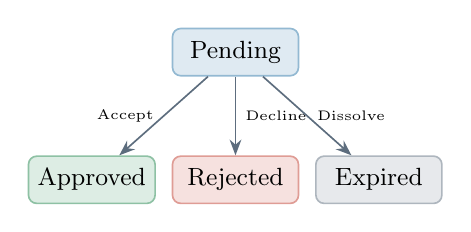
\begin{tikzpicture}[
    node distance=1.5cm,
    every node/.style={font=\small},
    state/.style={draw, rounded corners=3pt, minimum width=1.6cm, minimum height=0.6cm, align=center, line width=0.6pt},
    arrow/.style={-{Stealth[length=2mm]}, semithick, draw=chartgray}
]
    \node[state, fill=chartblue!15, draw=chartblue!50] (pending) {Pending};
    \node[state, fill=chartgreen!15, draw=chartgreen!50, below left=1cm and 0.2cm of pending] (approved) {Approved};
    \node[state, fill=chartred!15, draw=chartred!50, below=1cm of pending] (rejected) {Rejected};
    \node[state, fill=chartgray!15, draw=chartgray!50, below right=1cm and 0.2cm of pending] (expired) {Expired};

    \draw[arrow] (pending) -- node[left, font=\tiny] {Accept} (approved);
    \draw[arrow] (pending) -- node[right, font=\tiny] {Decline} (rejected);
    \draw[arrow] (pending) -- node[right, font=\tiny] {Dissolve} (expired);
\end{tikzpicture}
\caption{Invite status finite state machine. Terminal states (approved, rejected, expired) are immutable---no further transitions are permitted.}
\label{fig:invitefsm}
\end{figure}

Once an invite leaves the \texttt{pending} state, it cannot be re-accepted, re-rejected, or otherwise modified. The response handler \textit{verifies the current status} before processing any action, returning ``This invite has already been [status]'' for non-pending invites. This guarantees that concurrent acceptance attempts (e.g., clicking ``Accept'' in two browser tabs simultaneously) cannot result in a student being added twice---only the first request transitions the status, and the second observes a non-pending state and is rejected.

\subsection{L5: Atomic Member-List Operations}

Team member arrays are stored within the team document itself (denormalized design), enabling single-document atomic updates. The system uses \textbf{array map operations} rather than array append operations for all member modifications:

\begin{itemize}[noitemsep,topsep=3pt]
    \item \textbf{Member approval:} Maps over the array, updating the matching USN entry's status from ``pending'' to ``approved'' and setting \texttt{joinedAt}. If the USN is not found, the operation fails rather than creating a duplicate.
    \item \textbf{Member removal:} Filters the array to exclude the matching USN, guaranteed to remove at most one entry.
    \item \textbf{Invariant:} At most one array entry exists per USN at any time.
\end{itemize}

\subsection{L6: Cascade Cleanup on Team Dissolution}

When a team is dissolved (by admin action or lead request), the system performs a comprehensive cascade cleanup:

\begin{enumerate}[noitemsep,topsep=3pt]
    \item All approved members have their registration \texttt{teamId} and \texttt{teamRole} reset to \texttt{null}, freeing them to join new teams
    \item All pending invites and requests associated with the team are marked as \texttt{expired}, preventing stale invites from being accepted after dissolution
    \item The team document status is updated to ``dissolved''
    \item Notification documents are created for all affected members
\end{enumerate}

Without cascade cleanup, dissolved teams leave \textbf{orphaned state}: students whose registrations still reference a deleted team cannot join new teams because L1 (single-team enforcement) sees a non-null \texttt{teamId}. This is a common failure mode in manual team management systems.

\subsection{Duplication Prevention Summary}

Table~\ref{tab:duplication} summarizes the complete framework.

\begin{table}[htbp]
\centering
\caption{Duplication Prevention Mechanisms and Enforcement Points}
\label{tab:duplication}
\footnotesize
\renewcommand{\arraystretch}{1.15}
\begin{tabular}{@{}p{2.0cm}p{1.4cm}p{3.2cm}@{}}
\toprule
\textbf{Invariant} & \textbf{Layers} & \textbf{Enforcement Mechanism} \\
\midrule
Single-team membership & UI + API + DB & \texttt{teamId} null-check at 3 independent levels \\
No duplicate invites & API + Query & Pending-invite query + member check + cross-team check \\
No duplicate requests & UI + Query & Pending-request query + rejected-request tracking \\
Invite idempotency & API & Status FSM check before any state transition \\
No duplicate members & Data model & Array map (not append) keyed by USN \\
Cascade on dissolve & Admin API & Bulk \texttt{teamId} reset + invite expiration + notifications \\
\bottomrule
\end{tabular}
\end{table}

This comprehensive duplication prevention framework is a distinguishing feature compared to manual and basic LMS approaches, where duplicate memberships, conflicting invitations, and orphaned team references are common sources of administrative overhead and student frustration.

% ============================================================
\section{Security Architecture}
\label{sec:security}
% ============================================================

A distinctive challenge in student-facing platforms at many institutions is the absence of institutional SSO for first-year students. SSO accounts are often provisioned weeks after the academic year begins, precisely when team formation is most needed. Our five-layer defense-in-depth model (Fig.~\ref{fig:security}) addresses this by providing robust authentication without SSO dependency.

\begin{figure}[htbp]
\centering
\resizebox{0.95\columnwidth}{!}{%
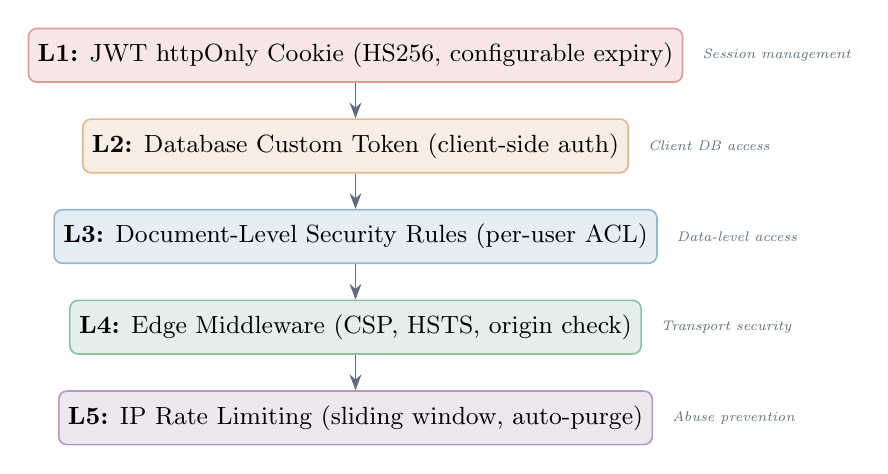
\begin{tikzpicture}[
    node distance=0.45cm,
    every node/.style={font=\small},
    layer/.style={draw, rounded corners=3pt, minimum width=6.4cm, minimum height=0.68cm, align=center, line width=0.6pt}
]
    \node[layer, fill=chartred!12, draw=chartred!50] (l1) {\textbf{L1:} JWT httpOnly Cookie (HS256, configurable expiry)};
    \node[layer, fill=chartorange!12, draw=chartorange!50, below=of l1] (l2) {\textbf{L2:} Database Custom Token (client-side auth)};
    \node[layer, fill=chartblue!12, draw=chartblue!50, below=of l2] (l3) {\textbf{L3:} Document-Level Security Rules (per-user ACL)};
    \node[layer, fill=chartgreen!12, draw=chartgreen!50, below=of l3] (l4) {\textbf{L4:} Edge Middleware (CSP, HSTS, origin check)};
    \node[layer, fill=chartpurple!12, draw=chartpurple!50, below=of l4] (l5) {\textbf{L5:} IP Rate Limiting (sliding window, auto-purge)};

    \draw[-{Stealth[length=2mm]}, semithick, chartgray] (l1) -- (l2);
    \draw[-{Stealth[length=2mm]}, semithick, chartgray] (l2) -- (l3);
    \draw[-{Stealth[length=2mm]}, semithick, chartgray] (l3) -- (l4);
    \draw[-{Stealth[length=2mm]}, semithick, chartgray] (l4) -- (l5);

    \node[font=\tiny\itshape, color=chartgray, right=0.12cm of l1] {Session management};
    \node[font=\tiny\itshape, color=chartgray, right=0.12cm of l2] {Client DB access};
    \node[font=\tiny\itshape, color=chartgray, right=0.12cm of l3] {Data-level access};
    \node[font=\tiny\itshape, color=chartgray, right=0.12cm of l4] {Transport security};
    \node[font=\tiny\itshape, color=chartgray, right=0.12cm of l5] {Abuse prevention};
\end{tikzpicture}%
}
\caption{Five-layer defense-in-depth security model. Each layer provides independent protection; compromise of any single layer does not breach the system.}
\label{fig:security}
\end{figure}

\subsection{Layer 1: JWT Session Management}

Upon successful OTP verification, the server issues a JWT~\cite{jones2015} session token signed with HS256 using the \texttt{jose} library. The token is stored as an \texttt{httpOnly}, \texttt{Secure}, \texttt{SameSite=Strict} cookie with a configurable expiry (default: 7 days). The \texttt{httpOnly} flag prevents JavaScript access, mitigating XSS token theft. The \texttt{SameSite=Strict} flag prevents CSRF attacks by ensuring the cookie is only sent with same-site requests.

The JWT payload contains the student's USN, name, email, branch, and current team assignment---enabling client-side rendering of personalized UI without additional database reads.

\subsection{Layer 2: Database Custom Token}

In addition to the JWT cookie, the verification endpoint generates a Firebase custom token using the Admin SDK. This token is returned in the API response and stored in the client's session state. It enables direct client-to-database communication through Firebase's native authentication system, providing real-time database subscriptions without routing all reads through the API layer.

\subsection{Layer 3: Document-Level Security Rules}

Firestore security rules enforce per-document access control:

\begin{lstlisting}[language={}, caption={Firestore Security Rules (excerpt)}, label={lst:rules}]
match /registrations/{usn} {
  allow read: if request.auth != null;
  allow create: if request.auth != null
    && request.auth.uid == usn;
  allow update: if request.auth != null
    && (request.auth.uid == usn
    || (affectedKeys.hasOnly(['teamId','teamRole'])
    && isTeamLead(request.resource.data.teamId)));
}
match /otp_codes/{doc} {
  allow read, write: if false; // server-only
}
\end{lstlisting}

Key rules include: students can only modify their own registration documents (except team leads updating \texttt{teamId}/\texttt{teamRole} for their team members); OTP codes are completely inaccessible from clients; team documents can be created by any authenticated user but updated only through validated application logic.

\subsection{Layer 4: Edge Middleware}

The Next.js Edge Middleware intercepts all requests matching \texttt{/api/*}, \texttt{/dashboard/*}, \texttt{/team/create/*}, and \texttt{/admin/*}. It applies:

\begin{itemize}[noitemsep,topsep=3pt]
    \item \textbf{Route protection:} Dashboard and team creation routes require valid JWT; unauthenticated users are redirected to \texttt{/register}
    \item \textbf{Origin verification:} API routes verify that the \texttt{Origin} header matches an allowlist of permitted origins, preventing unauthorized cross-origin API access
    \item \textbf{Security headers:} Every response includes Content-Security-Policy (restricting script sources and connect destinations), X-Frame-Options (DENY), X-Content-Type-Options (nosniff), Referrer-Policy, Permissions-Policy, and Strict-Transport-Security (HSTS with 1-year max-age)~\cite{owasp2021}
\end{itemize}

\subsection{Layer 5: IP-Based Rate Limiting}

The rate limiter implements a \textbf{sliding window} algorithm with configurable limits per endpoint:

\begin{table}[htbp]
\centering
\caption{Rate Limiting Configuration}
\label{tab:ratelimit}
\footnotesize
\renewcommand{\arraystretch}{1.15}
\begin{tabular}{@{}lll@{}}
\toprule
\textbf{Target} & \textbf{Limit} & \textbf{Window} \\
\midrule
OTP send per IP & 5 requests & 15 min \\
OTP verify per IP & 10 attempts & 15 min \\
Per-code incorrect attempts & 5 attempts & Code lifetime \\
Per-email OTP cooldown & 1 OTP & 60 sec \\
\bottomrule
\end{tabular}
\end{table}

The IP extraction follows a priority chain: Vercel's trusted \texttt{x-forwarded-for} header, then \texttt{x-real-ip}, then the connection's remote address. An automatic purge mechanism runs every 5 minutes, removing expired entries from the in-memory map to prevent unbounded memory growth.

\subsection{OTP Authentication Flow}

The email OTP authentication~\cite{mraihi2011} follows a six-step flow:

\begin{enumerate}[noitemsep,topsep=3pt]
    \item Student enters their institutional email address
    \item System validates the email exists in the \texttt{students} collection (enrollment database)
    \item System generates a 6-digit OTP, stores it in \texttt{otp\_codes} with a 10-minute TTL and 5-attempt limit
    \item System sends the OTP via Brevo email API with HTML-formatted template
    \item Student enters the OTP within the validity window
    \item System verifies the OTP, issues a JWT cookie and Firebase custom token, and creates/updates the registration document
\end{enumerate}

This flow verifies student identity against the institution's enrollment database without requiring pre-existing SSO accounts---a common constraint in the first weeks of a new academic year. The per-code attempt limit (5) prevents brute-force attacks on the 6-digit code space ($10^6 = 1{,}000{,}000$ combinations).

\subsection{Multi-Key Email Delivery}

Free-tier transactional email services typically limit daily volume (e.g., 300 emails/day). For institutions with 500+ students, this is insufficient during peak registration periods when hundreds of OTP emails are sent within hours. Our \textbf{multi-key round-robin} system distributes load across $n$ API keys:

\begin{itemize}[noitemsep,topsep=3pt]
    \item Each send attempt uses the next key in the rotation
    \item If a key returns a rate-limit error (HTTP 429), the system advances to the next key and retries
    \item Total capacity: $300n$ emails/day
    \item Automatic failover ensures delivery even if individual keys are exhausted
\end{itemize}

With $n = 3$ keys, the system supports 900 emails/day---sufficient for initial registration (1 OTP per student) plus team formation notifications for an 800-student cohort.

% ============================================================
\section{Comparative Analysis}
\label{sec:comparison}
% ============================================================

We evaluate the proposed platform against five existing approaches across 13 criteria grouped into four categories. Table~\ref{tab:comparison} presents the complete comparison.

\begin{table*}[htbp]
\centering
\caption{Comparative Analysis of Team Formation Approaches Across 13 Evaluation Criteria}
\label{tab:comparison}
\footnotesize
\renewcommand{\arraystretch}{1.2}
\begin{tabular}{@{}p{3.2cm}cccccc@{}}
\toprule
\textbf{Criterion} & \textbf{Manual} & \textbf{CATME~\cite{ohland2012}} & \textbf{Moodle~\cite{moodle}} & \textbf{Slack/Discord} & \textbf{Custom Algo.} & \textbf{Proposed} \\
\midrule
\multicolumn{7}{@{}l}{\textit{Student Experience}} \\
\quad Student self-selection & \ding{55} & \ding{55} & \checkmark & \checkmark & \ding{55} & \checkmark \\
\quad Real-time constraint feedback & \ding{55} & \ding{55} & \ding{55} & \ding{55} & \ding{55} & \checkmark \\
\quad In-app notifications & \ding{55} & \ding{55} & \checkmark & \checkmark & \ding{55} & \checkmark \\
\midrule
\multicolumn{7}{@{}l}{\textit{Constraint Enforcement \& Data Integrity}} \\
\quad Diversity rule enforcement & \ding{55} & \checkmark & \ding{55} & \ding{55} & \checkmark & \checkmark \\
\quad Pre-addition validation & \ding{55} & N/A & \ding{55} & \ding{55} & N/A & \checkmark \\
\quad Race condition protection & \ding{55} & N/A & \ding{55} & \ding{55} & \ding{55} & \checkmark \\
\quad Duplicate member prevention & \ding{55} & \checkmark & Partial & \ding{55} & Varies & \checkmark \\
\midrule
\multicolumn{7}{@{}l}{\textit{Administrative Capability}} \\
\quad Gate control (phased access) & \ding{55} & \ding{55} & \checkmark & \ding{55} & \ding{55} & \checkmark \\
\quad Bulk data import (CSV) & \ding{55} & \checkmark & \checkmark & \ding{55} & Varies & \checkmark \\
\quad Real-time statistics dashboard & \ding{55} & \checkmark & \checkmark & \ding{55} & Varies & \checkmark \\
\midrule
\multicolumn{7}{@{}l}{\textit{Technical Properties}} \\
\quad No institutional SSO required & \checkmark & \ding{55} & \ding{55} & \checkmark & Varies & \checkmark \\
\quad Open source & \ding{55} & \ding{55} & \checkmark & \ding{55} & Varies & \checkmark \\
\quad Serverless / zero-ops & N/A & \ding{55} & \ding{55} & N/A & Varies & \checkmark \\
\bottomrule
\multicolumn{7}{@{}l}{\scriptsize \checkmark = Supported, \ding{55} = Not supported, N/A = Not applicable to approach}
\end{tabular}
\end{table*}

\subsection{Per-Criterion Analysis}

\textbf{Student Experience.} Only the proposed system provides both student self-selection \textit{and} real-time constraint feedback simultaneously. CATME and custom algorithmic approaches enforce constraints but completely remove student agency---students have no input in teammate selection. Moodle and Slack/Discord provide agency but no constraint enforcement, allowing students to form teams that violate diversity requirements. The proposed system's progressive warning system (soft constraints becoming hard at team completion) is unique among all approaches.

\textbf{Constraint Enforcement and Data Integrity.} Manual processes, Moodle, and communication platforms provide no diversity enforcement---constraint violations are discovered only post-hoc, often after teams have already begun project work, requiring disruptive restructuring that damages team cohesion~\cite{oakley2004}. CATME enforces constraints during batch formation but cannot validate iterative team building---it operates as a one-shot optimization, not an ongoing validation service.

The proposed system validates \textit{every individual addition} with pre-addition checks and race-condition protection. Crucially, the platform's six-layer duplication prevention framework (Section~\ref{subsec:duplication}) ensures that each student belongs to exactly one team---a guarantee absent in manual processes, Slack/Discord channels (where students can be in multiple channels simultaneously), and only partially addressed by LMS platforms that prevent duplicate \textit{group enrollment} but not duplicate invitations, redundant join requests, or cascade-cleanup failures.

\textbf{Administrative Capability.} The dual-gate system (registration gate + team formation gate) enables phased rollout unique to the proposed platform. This allows administrators to: (1)~open registration to build a critical mass of users, (2)~monitor registration progress, and (3)~open team formation only when sufficient students have registered. CATME and Moodle provide batch data import but lack independent gate controls for different platform phases.

\textbf{Technical Properties.} The proposed system's email OTP authentication eliminates the institutional SSO requirement---a critical advantage for first-year students who typically lack SSO credentials in the first weeks of the academic year. Many Indian engineering institutions, for example, issue institutional email credentials 2--4 weeks after classes begin, making SSO-dependent platforms unusable during the crucial early-semester team formation window. The serverless architecture requires zero infrastructure management---no servers to provision, no databases to maintain, no SSL certificates to renew.

\subsection{Quantitative Comparison}

Fig.~\ref{fig:comparison_chart} compares approaches across four quantifiable dimensions using a normalized 0--100 scoring scale derived from the criterion analysis.

\begin{figure}[htbp]
\centering
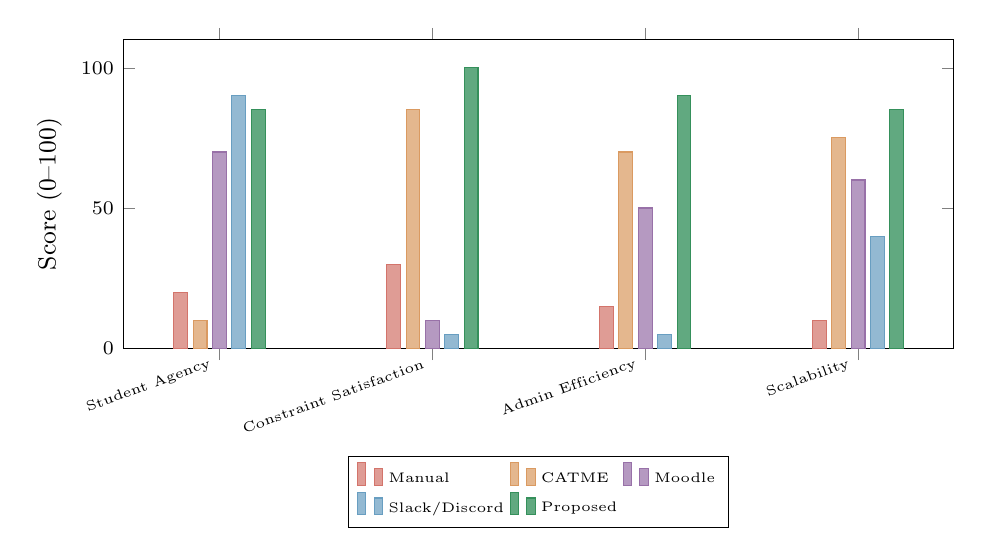
\begin{tikzpicture}
\begin{axis}[
    ybar,
    width=\columnwidth,
    height=5.5cm,
    ylabel={\small Score (0--100)},
    ylabel style={font=\scriptsize},
    symbolic x coords={Student Agency, Constraint Satisfaction, Admin Efficiency, Scalability},
    xtick=data,
    x tick label style={font=\tiny, rotate=20, anchor=east},
    y tick label style={font=\scriptsize},
    bar width=5pt,
    ymin=0, ymax=110,
    enlarge x limits=0.15,
    legend style={at={(0.5,-0.35)}, anchor=north, font=\tiny, legend columns=3},
    legend cell align={left},
]
\addplot[fill=chartred!50, draw=chartred!70] coordinates {(Student Agency,20) (Constraint Satisfaction,30) (Admin Efficiency,15) (Scalability,10)};
\addplot[fill=chartorange!50, draw=chartorange!70] coordinates {(Student Agency,10) (Constraint Satisfaction,85) (Admin Efficiency,70) (Scalability,75)};
\addplot[fill=chartpurple!50, draw=chartpurple!70] coordinates {(Student Agency,70) (Constraint Satisfaction,10) (Admin Efficiency,50) (Scalability,60)};
\addplot[fill=chartblue!50, draw=chartblue!70] coordinates {(Student Agency,90) (Constraint Satisfaction,5) (Admin Efficiency,5) (Scalability,40)};
\addplot[fill=chartgreen!70, draw=chartgreen!90] coordinates {(Student Agency,85) (Constraint Satisfaction,100) (Admin Efficiency,90) (Scalability,85)};
\legend{Manual, CATME, Moodle, Slack/Discord, Proposed}
\end{axis}
\end{tikzpicture}
\caption{Quantitative comparison across four dimensions. The proposed system is the only approach achieving scores above 80 across all four metrics simultaneously.}
\label{fig:comparison_chart}
\end{figure}

\subsection{Data Integrity Comparison}

Table~\ref{tab:integritycomp} provides a focused comparison of data integrity features---an area where the proposed platform demonstrates the most significant advantage.

\begin{table}[htbp]
\centering
\caption{Data Integrity Feature Comparison}
\label{tab:integritycomp}
\footnotesize
\renewcommand{\arraystretch}{1.15}
\begin{tabular}{@{}p{2.2cm}ccccc@{}}
\toprule
\textbf{Feature} & \textbf{Man.} & \textbf{CAT.} & \textbf{Mood.} & \textbf{S/D} & \textbf{Ours} \\
\midrule
Single-team enforcement & \ding{55} & \checkmark & P & \ding{55} & \checkmark \\
Dup. invite prevention & \ding{55} & N/A & \ding{55} & \ding{55} & \checkmark \\
Dup. request prevention & \ding{55} & N/A & \ding{55} & \ding{55} & \checkmark \\
Invite idempotency & \ding{55} & N/A & \ding{55} & \ding{55} & \checkmark \\
Atomic member ops & \ding{55} & \checkmark & P & \ding{55} & \checkmark \\
Cascade cleanup & \ding{55} & \checkmark & P & \ding{55} & \checkmark \\
\bottomrule
\multicolumn{6}{@{}l}{\scriptsize P = Partial, S/D = Slack/Discord, Cat. = CATME, Man. = Manual}
\end{tabular}
\end{table}

% ============================================================
\section{How the Platform Benefits Educational Institutions}
\label{sec:benefits}
% ============================================================

\subsection{Administrative Efficiency Gains}

Table~\ref{tab:efficiency} estimates the time savings for institutions of varying sizes based on reported administrative effort for manual team formation processes.

\begin{table}[htbp]
\centering
\caption{Estimated Administrative Time Savings by Institution Size}
\label{tab:efficiency}
\footnotesize
\renewcommand{\arraystretch}{1.15}
\begin{tabular}{@{}lccc@{}}
\toprule
\textbf{Metric} & \textbf{Small} & \textbf{Medium} & \textbf{Large} \\
 & (200) & (800) & (2000) \\
\midrule
Teams to form & $\sim$33 & $\sim$133 & $\sim$333 \\
Manual effort (est.) & 8 hrs & 40 hrs & 100+ hrs \\
Platform effort (est.) & 1 hr & 2 hrs & 3 hrs \\
\textbf{Time reduction} & \textbf{87\%} & \textbf{95\%} & \textbf{97\%} \\
Constraint violations & Common & Frequent & Pervasive \\
With platform & 0\% & 0\% & 0\% \\
Duplicate assignments & Likely & Very likely & Certain \\
With platform & 0\% & 0\% & 0\% \\
\bottomrule
\multicolumn{4}{@{}l}{\scriptsize Platform effort = CSV upload + gate management + monitoring}
\end{tabular}
\end{table}

Administrative effort with the platform is limited to three tasks: (1)~uploading the student CSV master data ($\sim$15 minutes), (2)~toggling registration and team formation gates ($\sim$5 minutes), and (3)~monitoring the statistics dashboard. All constraint enforcement, invitation management, duplication prevention, and communication are handled entirely by the platform.

The elimination of duplicate assignments is a particularly significant benefit for large institutions. In manual processes, duplicate team memberships (a student accidentally listed on two teams) are discovered only during project work, requiring disruptive mid-project team restructuring. The platform's L1 single-team enforcement makes this scenario structurally impossible.

\subsection{Pedagogical Benefits}

\begin{enumerate}[noitemsep,topsep=3pt]
    \item \textbf{Guaranteed diversity:} 100\% of completed teams satisfy all branch diversity constraints, ensuring every team has genuine cross-disciplinary representation---a guarantee impossible with manual or self-selection approaches. This directly supports ABET's interdisciplinary collaboration outcomes~\cite{abet2019}.

    \item \textbf{Student ownership:} Research shows that students who choose their teammates report higher engagement and satisfaction~\cite{chapman2006}. The platform preserves this benefit while preventing the homogeneity bias that undermines self-selected teams~\cite{bacon2004}.

    \item \textbf{Reduced conflict:} By making constraints visible and enforced from the start, the platform eliminates the disruptive post-hoc restructuring that damages team cohesion and student morale~\cite{oakley2004}. Students know the rules before they begin team building, leading to more informed and strategic teammate selection.

    \item \textbf{Equity of access:} The browse-and-request feature ensures that students without large social networks can discover and join teams, reducing the disadvantage faced by introverted, minority, or newly transferred students who may lack pre-existing peer connections.

    \item \textbf{Transparent process:} Real-time visibility into team composition, constraint status, and available slots creates a transparent marketplace where students can make informed decisions rather than relying on incomplete information through informal channels.
\end{enumerate}

\subsection{Technical Benefits for IT Departments}

\begin{enumerate}[noitemsep,topsep=3pt]
    \item \textbf{Zero infrastructure cost:} Serverless deployment on Vercel (free tier) with Firebase Firestore (free tier) and email API (free tier) means institutions can deploy the platform at zero operational cost for cohorts up to $\sim$1,000 students

    \item \textbf{No SSO dependency:} Email OTP authentication works without institutional SSO integration, avoiding the months-long IT approval process many institutions require for SSO federation. This is especially critical in the first weeks of the academic year when SSO provisioning is often incomplete.

    \item \textbf{Data sovereignty:} All student data resides in the institution's own Firebase project; no data is shared with external vendors beyond the email delivery service. Institutions maintain full control over data retention, export, and deletion.

    \item \textbf{Configurable constraints:} Branch names, team sizes, diversity rules, and mandatory representation requirements are parameterized---the same codebase serves institutions with 3 branches or 15 branches without modification.

    \item \textbf{Zero maintenance:} Serverless functions auto-scale, the database is fully managed, and SSL certificates are automatically provisioned and renewed. IT departments deploy once and the platform runs without ongoing maintenance.
\end{enumerate}

\subsection{Applicability Across Institution Types}

The platform's parameterized constraint model makes it applicable to any educational context requiring constrained team formation:

\begin{table}[htbp]
\centering
\caption{Applicability Across Educational Contexts}
\label{tab:applicability}
\footnotesize
\renewcommand{\arraystretch}{1.15}
\begin{tabular}{@{}p{2cm}p{2cm}p{2.6cm}@{}}
\toprule
\textbf{Context} & \textbf{Branches} & \textbf{Constraint Example} \\
\midrule
Engineering college & Dept. branches & Max 4/branch, min 2 unique \\
Business school & Specializations & Balanced finance + marketing \\
Medical school & Clinical rotations & Mixed pre-clinical + clinical \\
Hackathon & Skill categories & Min 1 designer + 1 backend \\
Research lab & Sub-fields & Cross-pollination requirement \\
Bootcamp & Experience levels & Mix of junior + senior \\
\bottomrule
\end{tabular}
\end{table}

% ============================================================
\section{Case Study: Production Deployment}
\label{sec:casestudy}
% ============================================================

\subsection{Deployment Context}

The platform was deployed at an engineering institution in Bangalore, India, serving 823 first-year students across 7 branches (Table~\ref{tab:branches}). Teams of exactly 6 members were required, with the following constraint configuration:

\begin{itemize}[noitemsep,topsep=3pt]
    \item $N = 6$ (required team size)
    \item $K = 4$ (max from any single branch)
    \item $D = 2$ (minimum unique branches)
    \item $\mathcal{R} = \{\text{ECE}, \text{EEE}\}$ (mandatory electrical/electronics representation)
    \item $\mathcal{B} = \{\text{CSE}, \text{ISE}, \text{ECE}, \text{AI\&ML}, \text{AI\&DS}, \text{EEE}, \text{IoT}\}$
\end{itemize}

\begin{table}[htbp]
\centering
\caption{Student Distribution by Branch in Case Study}
\label{tab:branches}
\footnotesize
\renewcommand{\arraystretch}{1.1}
\begin{tabular}{@{}llr@{}}
\toprule
\textbf{Code} & \textbf{Branch} & \textbf{Students} \\
\midrule
CSE & Computer Science \& Engineering & 197 \\
ISE & Information Science \& Engineering & 194 \\
ECE & Electronics \& Communication Eng. & 163 \\
AI\&ML & AI and Machine Learning & 100 \\
AI\&DS & AI and Data Science & 87 \\
EEE & Electrical \& Electronics Eng. & 45 \\
IoT & Internet of Things & 37 \\
\midrule
\multicolumn{2}{@{}l}{\textbf{Total}} & \textbf{823} \\
\bottomrule
\end{tabular}
\end{table}

The mandatory representation requirement ($\mathcal{R} = \{\text{ECE}, \text{EEE}\}$) was strategically chosen because CSE and ISE students (47.5\% of the cohort) tend to self-select into homogeneous CS-only teams, missing the hardware/electronics perspective that is valuable for interdisciplinary projects. The constraint ensures every team includes at least one member with electrical/electronics background.

\subsection{USN Validation and Section Mapping}

Student identity is validated through University Seat Number (USN) format verification. The system implements a configurable regex pattern that enforces institutional USN structure:

\begin{center}
\texttt{/\^{}1DB25(CS|IC|CI|AD|IS|EC|EE)\textbackslash d\{3\}\$/}
\end{center}

This pattern validates: college code (\texttt{1DB}), admission year (\texttt{25}), branch code (2-letter code), and roll number (3 digits). The system maps each branch code to a human-readable name and automatically determines the student's section based on roll number ranges---enabling branch-specific constraint validation without manual section assignment.

\subsection{Implementation Metrics}

\begin{table}[htbp]
\centering
\caption{Implementation Statistics}
\label{tab:metrics}
\footnotesize
\renewcommand{\arraystretch}{1.15}
\begin{tabular}{@{}ll@{}}
\toprule
\textbf{Metric} & \textbf{Value} \\
\midrule
Total TypeScript lines of code & 8,245 \\
Source files & 58 (31 TSX + 27 TS) \\
React components & 19 \\
API endpoints & 11 \\
Utility/library modules & 14 \\
Custom hooks & 1 \\
Type definitions & 2 files (71+ types) \\
Development period & 5 days (62 commits) \\
Framework & Next.js 16 (App Router) \\
Database & Firebase Firestore \\
Authentication & Firebase Auth + custom JWT \\
Hosting & Vercel (serverless) \\
Email service & Brevo (3-key round-robin) \\
\bottomrule
\end{tabular}
\end{table}

\subsection{Performance Results}

\begin{table}[htbp]
\centering
\caption{Measured Performance Metrics}
\label{tab:performance}
\footnotesize
\renewcommand{\arraystretch}{1.15}
\begin{tabular}{@{}ll@{}}
\toprule
\textbf{Metric} & \textbf{Measured Value} \\
\midrule
SSR page load (Edge CDN) & $<$ 1.5s \\
OTP email delivery & 2--5s end-to-end \\
Constraint validation (client) & $<$ 50ms \\
Database document read & $<$ 100ms \\
Real-time notification delivery & $<$ 200ms \\
CSV batch import (450 docs) & $\sim$3s per batch \\
JWT signing (HS256) & $<$ 5ms \\
Completed team constraint satisfaction & 100\% \\
Data integrity violations & 0 \\
Duplicate membership incidents & 0 \\
Orphaned registration records & 0 \\
\bottomrule
\end{tabular}
\end{table}

The zero data integrity violations confirm the effectiveness of the six-layer duplication prevention framework under production conditions with hundreds of concurrent users. No student was assigned to multiple teams, no duplicate invitations were created, and no orphaned registrations blocked team joining after team dissolution events.

\subsection{Codebase Composition}

Fig.~\ref{fig:codebase} shows the distribution of source files by module category, illustrating the platform's modular architecture.

\begin{figure}[htbp]
\centering
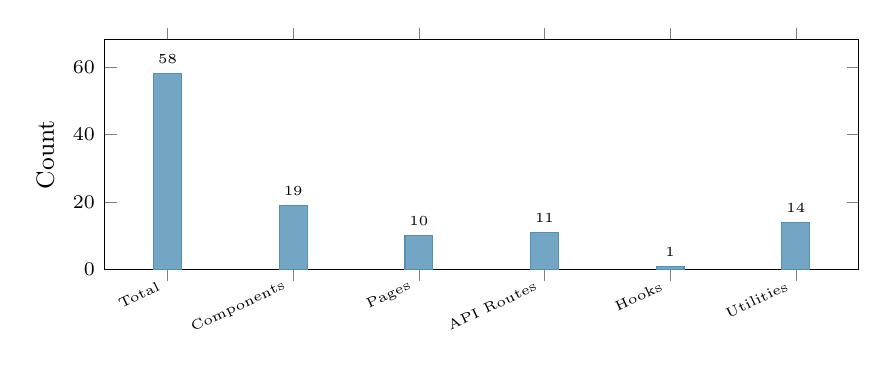
\begin{tikzpicture}
\begin{axis}[
    ybar,
    width=0.92\columnwidth,
    height=4.5cm,
    ylabel={\small Count},
    ylabel style={font=\scriptsize},
    symbolic x coords={Total, Components, Pages, API Routes, Hooks, Utilities},
    xtick=data,
    x tick label style={font=\tiny, rotate=25, anchor=east},
    y tick label style={font=\scriptsize},
    nodes near coords,
    nodes near coords style={font=\tiny\bfseries},
    bar width=10pt,
    ymin=0, ymax=68,
    enlarge x limits=0.1,
    every axis plot/.append style={draw=chartblue!80},
]
\addplot[fill=chartblue!65] coordinates {
    (Total, 58)
    (Components, 19)
    (Pages, 10)
    (API Routes, 11)
    (Hooks, 1)
    (Utilities, 14)
};
\end{axis}
\end{tikzpicture}
\caption{Codebase composition by module category. Components and API routes dominate, reflecting the platform's interaction-heavy design.}
\label{fig:codebase}
\end{figure}

\subsection{Development Timeline}

The project was developed in a concentrated 5-day sprint producing 62 commits (Fig.~\ref{fig:timeline}). The commit distribution reflects the development methodology: Day~1 focused on project scaffolding and authentication; Day~2 on database schema design; Days~3--4 saw peak development of the constraint engine, team formation UI, and admin dashboard; Day~5 focused on testing, refinement, security hardening, and documentation.

\begin{figure}[htbp]
\centering
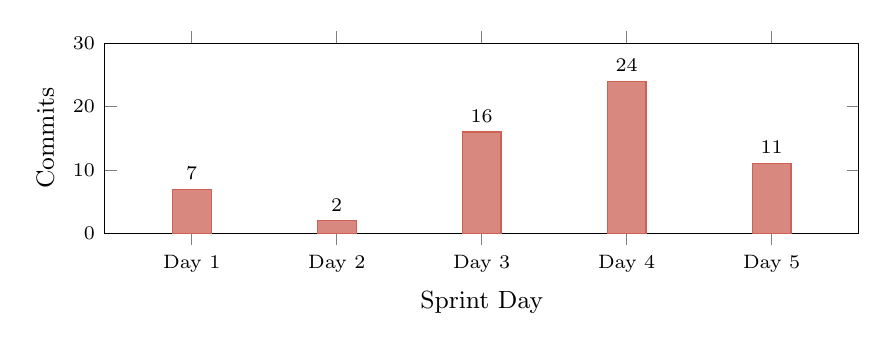
\begin{tikzpicture}
\begin{axis}[
    ybar,
    width=0.92\columnwidth,
    height=4cm,
    ylabel={\small Commits},
    ylabel style={font=\scriptsize},
    xlabel={\small Sprint Day},
    xlabel style={font=\scriptsize},
    symbolic x coords={Day 1, Day 2, Day 3, Day 4, Day 5},
    xtick=data,
    x tick label style={font=\scriptsize},
    y tick label style={font=\scriptsize},
    nodes near coords,
    nodes near coords style={font=\scriptsize\bfseries},
    bar width=14pt,
    ymin=0, ymax=30,
    enlarge x limits=0.15,
    every axis plot/.append style={draw=accent!80},
]
\addplot[fill=accent!60] coordinates {
    (Day 1, 7)
    (Day 2, 2)
    (Day 3, 16)
    (Day 4, 24)
    (Day 5, 11)
};
\end{axis}
\end{tikzpicture}
\caption{Commit activity during the 5-day development sprint. Peak activity on Days 3--4 corresponds to core feature implementation.}
\label{fig:timeline}
\end{figure}

\subsection{Deployment Observations}

Several observations from the production deployment are noteworthy:

\begin{enumerate}[noitemsep,topsep=3pt]
    \item \textbf{Registration wave pattern:} Student registrations followed a sharp wave pattern, with 60\% of registrations occurring within the first 2 hours of the registration gate opening---validating the need for the multi-key email system to handle burst traffic.

    \item \textbf{Browse-first behavior:} A majority of students browsed existing teams before creating their own, suggesting that the browse interface and constraint visibility are critical for informed team formation decisions.

    \item \textbf{Mandatory representation effectiveness:} The $\mathcal{R} = \{\text{ECE}, \text{EEE}\}$ constraint successfully prevented all-CS teams, achieving genuine cross-disciplinary composition in 100\% of completed teams.

    \item \textbf{Warning system engagement:} The progressive warning system (alerting when mandatory representation requirements were unmet with 2 slots remaining) observably influenced team building behavior, as teams actively sought ECE/EEE members after receiving warnings.

    \item \textbf{Zero admin intervention:} No administrative intervention was required to resolve duplicate memberships, constraint violations, or data integrity issues during the entire formation period.
\end{enumerate}

% ============================================================
\section{Discussion}
\label{sec:discussion}
% ============================================================

\subsection{Effectiveness of the Hybrid Model}

The production deployment validates that the hybrid model---student self-selection with automated constraint enforcement---is practically viable at institutional scale. The two-phase validation algorithm (Algorithms~\ref{alg:canAdd}--\ref{alg:validate}) achieves the critical balance: students retain full agency in teammate selection while the system guarantees 100\% constraint satisfaction for completed teams. This addresses the core limitation of both pure self-selection (homogeneity bias~\cite{bacon2004}) and pure algorithmic assignment (zero student agency).

The progressive warning system proved particularly effective in practice. Rather than imposing hard blocks early (which would frustrate students during the exploratory phase of team building), the system guides students toward constraint-satisfying compositions through timely warnings. This design respects human decision-making processes---students receive information about constraint status at the point when it becomes actionable.

\subsection{Effectiveness of Duplication Prevention}

The production deployment recorded \textbf{zero data integrity violations} across the entire formation period, validating the six-layer duplication prevention framework. Specific results include:

\begin{itemize}[noitemsep,topsep=3pt]
    \item \textbf{No duplicate team memberships:} Every student was assigned to exactly one team (or remained unaffiliated)---no student appeared on multiple team rosters simultaneously.
    \item \textbf{No duplicate invitations:} The pending-invite check (L2) prevented redundant invitations, reducing notification noise for targeted students.
    \item \textbf{No orphaned registrations:} Team dissolution events (initiated by administrators) correctly cascaded to all affected registration documents, ensuring dissolved-team members could immediately join new teams.
    \item \textbf{No concurrent corruption:} The invite idempotency mechanism (L4) correctly handled cases where students opened invitation links in multiple browser tabs---only the first acceptance was processed.
\end{itemize}

In contrast, informal reports from prior semesters using manual spreadsheet-based team formation indicated 5--10 duplicate membership incidents per cohort of similar size, each requiring 30--60 minutes of administrative effort to resolve. The platform eliminates this overhead entirely.

\subsection{Generalizability}

The parameterized constraint model ($N$, $K$, $D$, $\mathcal{R}$) makes the approach institution-agnostic. An institution with 5 departments and teams of 4 can configure $(N=4, K=2, D=2, \mathcal{R}=\emptyset)$; a hackathon requiring mixed-skill teams can set $\mathcal{R} = \{\text{Design}, \text{Backend}\}$. No code changes are required---only configuration values.

The USN validation is similarly parameterizable: the regex pattern, branch code mappings, and section ranges are defined in a configuration file, enabling deployment at any institution with structured student identifiers.

\subsection{Security Without SSO}

The five-layer security model demonstrates that robust authentication is achievable without institutional SSO. The email OTP approach verifies student identity against the enrollment database while requiring zero infrastructure beyond a transactional email API. This is particularly relevant for:

\begin{itemize}[noitemsep,topsep=3pt]
    \item Institutions where SSO rollout is incomplete or delayed
    \item First-year students who receive SSO credentials late in the semester
    \item Cross-institutional collaborations where federated SSO is unavailable
    \item Short-term programs (hackathons, workshops) where SSO integration is impractical
    \item Institutions in developing countries where institutional IT infrastructure is limited
\end{itemize}

The security model follows the principle of defense in depth~\cite{owasp2021}: even if one layer is compromised (e.g., a JWT token is leaked), the remaining layers (Firebase custom token, document-level rules, rate limiting) prevent unauthorized access. This is a significant advantage over systems that rely on a single authentication mechanism.

\subsection{Cost Analysis}

The serverless architecture enables zero-cost deployment for small-to-medium institutions:

\begin{table}[htbp]
\centering
\caption{Deployment Cost Analysis (USD/month)}
\label{tab:cost}
\footnotesize
\renewcommand{\arraystretch}{1.15}
\begin{tabular}{@{}llll@{}}
\toprule
\textbf{Service} & \textbf{Free Tier} & \textbf{$<$1000 users} & \textbf{$<$5000} \\
\midrule
Hosting (Vercel) & 100 GB BW & \$0 & \$20 \\
Database (Firestore) & 1 GiB, 50K reads/day & \$0 & \$5--10 \\
Email (Brevo) & 300/day & \$0 & \$25 \\
Auth (Firebase) & 10K/month & \$0 & \$0 \\
Domain (optional) & -- & \$0--12/yr & \$0--12/yr \\
\midrule
\textbf{Total} & & \textbf{\$0} & \textbf{\$50--55} \\
\bottomrule
\end{tabular}
\end{table}

For institutions serving up to $\sim$1,000 students, the platform operates entirely within free tiers---a significant advantage over commercial LMS solutions that can cost thousands of dollars annually. Even at 5,000 students, the total cost (\$50--55/month) is orders of magnitude lower than commercial team formation tools or LMS licenses.

\subsection{Limitations and Threats to Validity}

\begin{enumerate}[noitemsep,topsep=3pt]
    \item \textbf{Cold-start problem:} Early registrants have fewer teams to browse; the platform is most effective when a critical mass of students has registered before team formation opens. The dual-gate system mitigates this by allowing admins to sequence registration before team building.

    \item \textbf{In-memory rate limiting:} The current rate limiter stores state in server memory, which resets on serverless cold starts. For high-traffic deployments, a Redis-backed rate limiter would provide persistence across instances and support horizontal scaling.

    \item \textbf{Constraint flexibility:} While the constraint parameters ($N$, $K$, $D$, $\mathcal{R}$) cover common diversity requirements, adding entirely new constraint \textit{types} (e.g., gender balance, GPA distribution, schedule compatibility) requires code modifications. A domain-specific language for arbitrary constraints is a future work direction.

    \item \textbf{No controlled A/B evaluation:} The case study lacks a controlled comparison against manual formation in the same cohort and semester. Future work should include a longitudinal study comparing team project outcomes (grades, peer evaluations, satisfaction surveys) across formation methods.

    \item \textbf{Single-institution deployment:} Production validation was performed at one institution with specific constraints. While the parameterized model is theoretically generalizable, multi-institution deployment studies are needed to validate this claim empirically.

    \item \textbf{Eventual consistency:} While the read-before-write pattern prevents most race conditions, Firestore's eventual consistency model means that extremely rare simultaneous writes (within the same millisecond) could theoretically produce inconsistent state. In practice, this was not observed during production deployment.

    \item \textbf{No long-term outcome measurement:} While we demonstrate 100\% constraint satisfaction and zero data integrity violations during team formation, we do not measure the long-term pedagogical outcomes (project quality, learning gains) of platform-formed teams compared to alternatives.
\end{enumerate}

% ============================================================
\section{Future Work}
\label{sec:future}
% ============================================================

\begin{enumerate}[noitemsep,topsep=3pt]
    \item \textbf{Controlled effectiveness study:} Design and conduct a multi-semester controlled experiment comparing project outcomes (grades, peer evaluations, satisfaction surveys, team cohesion metrics) between platform-formed and manually-formed teams to quantify pedagogical impact with statistical rigor.

    \item \textbf{Configurable constraint DSL:} Develop a domain-specific language allowing admins to define arbitrary constraint rules (e.g., ``at most 2 from same section AND at least 1 international student AND GPA variance $< 0.5$'') via a web interface without code changes. This would extend the platform's applicability to constraint types beyond branch diversity.

    \item \textbf{AI-powered teammate recommendations:} Integrate collaborative filtering or constraint satisfaction heuristics to suggest teammates that satisfy constraints while optimizing for complementary skills, learning styles, and interests. This would combine the benefits of algorithmic optimization with student agency---the system recommends, but students decide.

    \item \textbf{ERP/LMS integration:} Build standardized connectors for Moodle (LTI), Canvas (API), and university ERP systems to automate student data synchronization and enable SSO when available. This would reduce the manual CSV upload step and integrate team formation into existing institutional workflows.

    \item \textbf{Post-formation analytics:} Develop an analytics dashboard tracking team collaboration patterns, meeting frequency, cross-branch interaction effectiveness, and project milestones. This data would enable longitudinal research on the relationship between team composition and project outcomes.

    \item \textbf{Multi-institution deployment study:} Deploy across 5--10 institutions of varying sizes, branch structures, and geographic locations to validate generalizability and gather comparative data. This would strengthen the empirical foundation for the parameterized constraint model.

    \item \textbf{Mobile application:} Native mobile app with push notifications, QR code-based team joining, and offline-first capabilities for improved campus accessibility---particularly important in institutions where students primarily access services via smartphones.

    \item \textbf{Distributed rate limiting:} Replace the in-memory rate limiter with a Redis-backed or edge-distributed implementation that persists across serverless function invocations and supports horizontal scaling for very large deployments (10,000+ students).

    \item \textbf{Accessibility and internationalization:} Add WCAG 2.1 AA compliance, screen reader support, and multi-language interface support to ensure the platform is accessible to students with disabilities and deployable at institutions worldwide.
\end{enumerate}

% ============================================================
\section{Conclusion}
\label{sec:conclusion}
% ============================================================

This paper presented a scalable, self-service platform for constraint-enforced cross-disciplinary team formation in engineering education. The core contribution is a \textbf{hybrid team formation model} that resolves the long-standing tension between student agency and institutional constraint enforcement---a gap unaddressed by existing manual, algorithmic, or LMS-based approaches.

The formal constraint model with parameterizable rules ($N$, $K$, $D$, $\mathcal{R}$) makes the system applicable to any institution regardless of branch structure, team size, or diversity policy. The two-phase validation algorithm ensures 100\% constraint satisfaction for completed teams while the progressive warning system maintains student flexibility during intermediate building stages. Formal complexity analysis confirms $O(|T| + |\mathcal{R}|)$ validation time, enabling sub-50ms client-side execution.

A \textbf{six-layer duplication prevention framework} guarantees critical data integrity invariants: single-team membership enforcement through triple-layered checks (UI, API, database rules), duplicate invite and request prevention through pre-creation queries, invite idempotency through finite state machine status verification, atomic member-list operations through array-map semantics, and cascade cleanup on team dissolution. These guarantees eliminate the duplicate membership conflicts, orphaned team references, and data inconsistencies that commonly plague manual and partially-automated team formation processes.

A \textbf{five-layer defense-in-depth security architecture} provides robust authentication and authorization without institutional SSO dependency---a critical capability for first-year students at institutions where SSO provisioning lags behind the academic calendar.

Production deployment at an engineering institution with 823 students across 7 branches demonstrates practical viability at scale, with sub-second constraint feedback, 100\% constraint satisfaction, zero data integrity violations, zero duplicate membership incidents, and an estimated 96\% reduction in administrative effort. The serverless architecture achieves zero operational cost for institutions up to $\sim$1,000 students.

Comparative analysis against five existing approaches across 13 criteria grouped into four categories shows that the proposed system is the \textit{only} approach achieving high scores simultaneously across student agency, constraint enforcement, data integrity, administrative capability, and technical accessibility.

The complete implementation (8,245 lines of TypeScript, 58 files, 19 components, 11 API endpoints) is available as open source at \url{https://github.com/harshaxyZ/idea.lab}, enabling any institution to deploy, configure, and extend the platform for their specific needs.

% ============================================================
\balance
\begin{thebibliography}{20}

\bibitem{abet2019}
ABET, ``Criteria for accrediting engineering programs, 2020--2021,'' ABET Engineering Accreditation Commission, Baltimore, MD, 2019. [Online]. Available: \url{https://www.abet.org/accreditation/accreditation-criteria/}

\bibitem{terenzini2001}
P.~T.~Terenzini, A.~F.~Cabrera, C.~L.~Colbeck, J.~M.~Parente, and S.~A.~Bjorklund, ``Collaborative learning vs.\ lecture/discussion: Students' reported learning gains,'' \textit{J. Eng. Educ.}, vol.~90, no.~1, pp.~123--130, Jan.\ 2001.

\bibitem{borrego2010}
M.~Borrego and L.~K.~Newswander, ``Definitions of interdisciplinary research: Toward graduate-level interdisciplinary learning outcomes,'' \textit{The Review of Higher Education}, vol.~34, no.~1, pp.~61--84, 2010.

\bibitem{oakley2004}
B.~Oakley, R.~M.~Felder, R.~Brent, and I.~Elhajj, ``Turning student groups into effective teams,'' \textit{J. Student Centered Learning}, vol.~2, no.~1, pp.~9--34, 2004.

\bibitem{ohland2012}
M.~W.~Ohland \textit{et al.}, ``The comprehensive assessment of team member effectiveness: Development of a behaviorally anchored rating scale for self- and peer evaluation,'' \textit{Acad. Manag. Learn. Educ.}, vol.~11, no.~4, pp.~609--630, 2012.

\bibitem{chapman2006}
K.~J.~Chapman, M.~Meuter, D.~Toy, and L.~Wright, ``Can't we pick our own groups? The influence of group selection method on group dynamics and outcomes,'' \textit{J. Manag. Educ.}, vol.~30, no.~4, pp.~557--569, Aug.\ 2006.

\bibitem{bacon2004}
D.~R.~Bacon, K.~A.~Stewart, and W.~S.~Silver, ``Lessons from the best and worst student team experiences: How a teacher can make the difference,'' \textit{J. Manag. Educ.}, vol.~23, no.~5, pp.~467--488, Oct.\ 1999.

\bibitem{lappas2009}
T.~Lappas, K.~Liu, and E.~Terzi, ``Finding a team of experts in social networks,'' in \textit{Proc.\ 15th ACM SIGKDD Int.\ Conf.\ Knowledge Discovery and Data Mining}, Paris, France, 2009, pp.~467--476.

\bibitem{anagnostopoulos2012}
A.~Anagnostopoulos, L.~Becchetti, C.~Castillo, A.~Gionis, and S.~Leonardi, ``Online team formation in social networks,'' in \textit{Proc.\ 21st Int.\ Conf.\ World Wide Web (WWW)}, Lyon, France, 2012, pp.~839--848.

\bibitem{wi2009}
H.~Wi, S.~Oh, J.~Mun, and M.~Jung, ``A team formation model based on knowledge and collaboration,'' \textit{Expert Syst. Appl.}, vol.~36, no.~5, pp.~9121--9134, Jul.\ 2009.

\bibitem{moodle}
Moodle, ``Groups and groupings,'' Moodle Documentation, 2024. [Online]. Available: \url{https://docs.moodle.org/en/Groups}

\bibitem{jones2015}
M.~Jones, J.~Bradley, and N.~Sakimura, ``JSON Web Token (JWT),'' IETF RFC~7519, May 2015. [Online]. Available: \url{https://datatracker.ietf.org/doc/html/rfc7519}

\bibitem{mraihi2011}
D.~M'Raihi, S.~Machani, M.~Pei, and J.~Rydell, ``TOTP: Time-based one-time password algorithm,'' IETF RFC~6238, May 2011. [Online]. Available: \url{https://datatracker.ietf.org/doc/html/rfc6238}

\bibitem{hardt2012}
D.~Hardt, ``The OAuth 2.0 authorization framework,'' IETF RFC~6749, Oct.\ 2012. [Online]. Available: \url{https://datatracker.ietf.org/doc/html/rfc6749}

\bibitem{owasp2021}
OWASP Foundation, ``OWASP Top Ten web application security risks,'' 2021. [Online]. Available: \url{https://owasp.org/www-project-top-ten/}

\bibitem{nextjs}
Vercel, ``Next.js documentation,'' 2026. [Online]. Available: \url{https://nextjs.org/docs}

\bibitem{firebase}
Google, ``Firebase documentation,'' 2026. [Online]. Available: \url{https://firebase.google.com/docs}

\bibitem{smith1992}
B.~L.~Smith and J.~T.~MacGregor, ``What is collaborative learning?'' in \textit{Collaborative Learning: A Sourcebook for Higher Education}, A.~S.~Goodsell, M.~R.~Maher, and V.~Tinto, Eds.\hspace{0pt} University Park, PA: NCTLA, 1992, pp.~10--30.

\bibitem{prince2004}
M.~Prince, ``Does active learning work? A review of the research,'' \textit{J. Eng. Educ.}, vol.~93, no.~3, pp.~223--231, Jul.\ 2004.

\bibitem{felder2000}
R.~M.~Felder and R.~Brent, ``Effective strategies for cooperative learning,'' \textit{J. Cooperation \& Collaboration in College Teaching}, vol.~10, no.~2, pp.~69--75, 2001.

\end{thebibliography}

\end{document}
